\chapter{Normally hyperbolic invariant manifolds}
The objective of this chapter is to extend the theory of low-dimensional stable and unstable manifolds to a general, higher-dimensional setting. The focus will lie on invariant manifolds rather than individual trajectories as invariant manifolds are more observable, more influential, and more robust. We begin with an example.

\begin{ex}[Dynamics near a saddle-type fixed point]
	The difference between the behavior of individual trajectories and of the invariant manifolds is depicted in Fig. \ref{fig:individual_trajectory}. The idea being that under a diffeomorphic transformation of the invariant manifolds of the linear system into those of the nonlinear system, a trajectory starting from a point $x_0$ may be drastically different even if the dynamics remain topologically conjugate to each other. I.e. individual trajectories are sensitive with respect to initial conditions and changes in parameters, meanwhile robust invariant manifolds persist (perturb smoothly).
	\begin{figure}[h!]
		\centering
		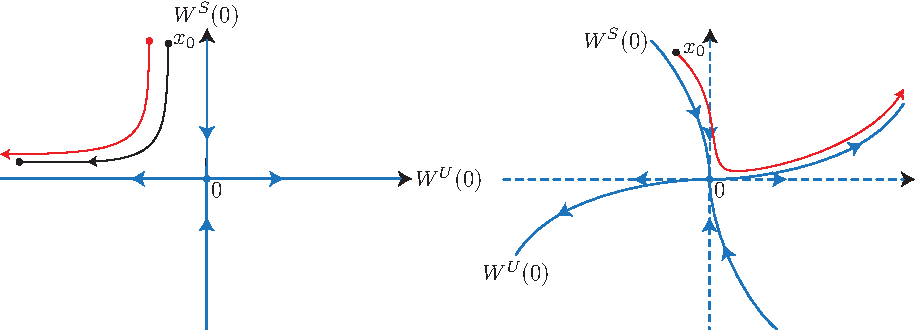
\includegraphics[width=0.99\textwidth]{figures/ch9/1individual_trajectory.pdf}
		\caption{The dynamics near a saddle-type fixed point demonstrating the sensitive dependence of individual trajectories on initial conditions and changes in parameters, and the robust nature of invariant manifolds.}
		\label{fig:individual_trajectory}
	\end{figure}
\end{ex}

Thus our examination now turns to determining which invariant manifolds are persistent. In order to understand this, first an intermezzo in differentiable manifolds is necessary.

\section{A crash course on differentiable manifolds}
\begin{definition}
	A set $M\subset \mathbb{R}^{n}$ is a \emph{$k$-dimensional differentiable manifold}, if it is \underline{locally} diffeomorphic to $\mathbb{R}^{k}$, i.e. for every $x\in M$ there exists an open (in $M$) neighborhood $V\subset M $, such that $V$ is diffeomorphic to an open set $U \subset \mathbb{R}^{k}$. The diffeomorphism is called the \emph{local parameterization} as is denoted $\Phi:U \to V$. Its smooth inverse is the \emph{local coordinate system} $\Phi^{-1}:V \to U$. These are illustrated in Fig. \ref{fig:diffble_mfd}.
	\begin{figure}[h!]
		\centering
		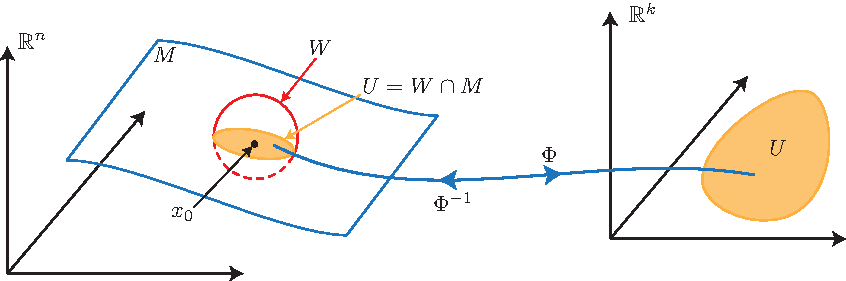
\includegraphics[width=0.99\textwidth]{figures/ch9/2diffble_mfd.pdf}
		\caption{The differentiable manifold $M$ is given in blue in the left. The red sphere $W$ is an open ball in  $\mathbb{R}^{n}$, intersecting this with $M$ yields and open (in $M$) neighborhood $V=W \cap M$ of $x $. The smooth diffeomorphism $\Phi $ transforms $U$ into the open set $U$ of $\mathbb{R}^{k}$.}
		\label{fig:diffble_mfd}
	\end{figure}
\end{definition}

The intuitive meaning of a $k$-dimensional manifold is a set which locally looks like $\mathbb{R}^{k}$.

\begin{definition}
	For a set $M\subset \mathbb{R}^{n}$ and an open set $U\subset \mathbb{R}^{n}$, the set $M\cap U$ is called \emph{relatively open} in $M$.	
\end{definition}

\begin{ex}[The circle is a 1-dimensional manifold]
	The circle $\mathcal{S}^{1}$ is a 1-dimensional differentiable manifold. To see define the four open subsets $V_i$ of $\mathcal{S}^{1}$ as open semicircles which are each shifted by $\frac{i \pi }{2} $ for $i=1,2,3,4$. Then $\mathcal{S}^{1} = \bigcup_{i=1}^{4}V_i$. These are drawn in Fig. \ref{fig:s1_subsets}. Any $x\in \mathcal{S}^{1}$ belongs to at least one of the $V_i$ due to the previous equality. Furthermore each $V_i$ is diffeomorphic to $U=(-1,1)$ which is open in $\mathbb{R}^{1}$ via the diffeomorphisms
	\begin{subequations}
		\begin{align}
		\Phi_1 &= 
		\begin{pmatrix}
			t\\ \sqrt{1-t^2}
		\end{pmatrix}
		;&&\Phi_2 = 
		\begin{pmatrix}
			t\\ -\sqrt{1-t^2}
		\end{pmatrix}
		; \\
		\Phi_3 &= 
		\begin{pmatrix}
			-\sqrt{1-t^2}\\ t
		\end{pmatrix}
		;&&\Phi_4 = 
		\begin{pmatrix}
			\sqrt{1-t^2}\\ t
		\end{pmatrix}
		.
		\end{align}
	\end{subequations}
\begin{figure}[h!]
	\centering
	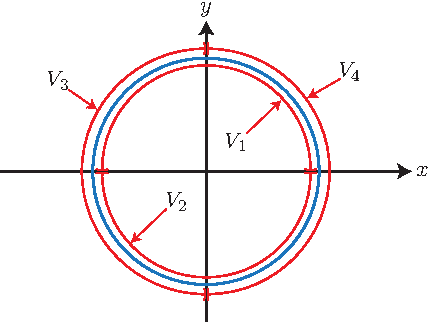
\includegraphics[width=0.6\textwidth]{figures/ch9/3s1_subsets.pdf}
	\caption{The subsets $V_i$ of $\mathcal{S}^{1} $ which are used to show that the circle is a 1-dimensional manifold.}
	\label{fig:s1_subsets}
\end{figure}

There is no global parameterization of $\mathcal{S}^{1}$, but this is not needed to be a differentiable manifold, and these local parameterizations suffice.	
\end{ex}

\begin{ex}[Not all sets are manifolds]
	A few examples of sets which are not manifolds.
	\begin{enumerate}
		\item The figure-eight is not a manifold, as for any point except the central intersection, there exists a local neighborhood diffeomorphic to $\mathbb{R}^{1}$, however at this central intersection, no open neighborhood exists which is diffeomorphic to $\mathbb{R}^{1}$. This is depicted in Fig. \ref{fig:figure_eight}.
			\begin{figure}[h!]
				\centering
				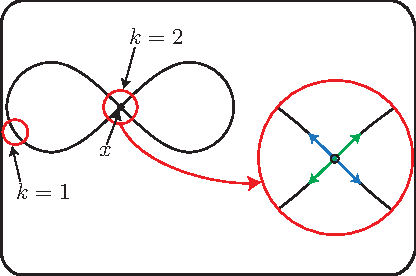
\includegraphics[width=0.6\textwidth]{figures/ch9/3b_figure_eight.pdf}
				\caption{The figure-eight with the critical intersection which prevents it from being a manifold.}
				\label{fig:figure_eight}
			\end{figure}
		\item A dense orbit on a 2-dimensional torus is not a manifold, as around any point infinitely many adjacent trajectories exist, but do not form a plane (there is a distance between two instances of the trajectory). Hence any neighborhood around any point cannot be hyperbolic to $\mathbb{R}^{2}$ or $\mathbb{R}^{1}$. Such a neighborhood is illustrated in Fig. \ref{fig:dense_orbit_mfd}.
			\begin{figure}[h!]
				\centering
				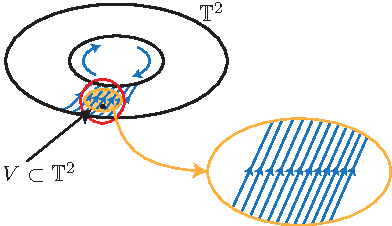
\includegraphics[width=0.6\textwidth]{figures/ch9/4dense_orbits_mfd.pdf}
				\caption{A depiction of a local neighborhood of a point in a dense orbit of the torus.}
				\label{fig:dense_orbit_mfd}
			\end{figure}
		\item The union of a semi-infinite spiral and semi-open (left closed, right open) interval do not form a differentiable manifold. For this set, at the intersections of the two sets, points with neighborhoods as in the figure eight appear.
	\end{enumerate}
\end{ex}

We can construct manifolds very easily, for instance by taking any smooth function $f:X \to Y$, the graph of $f$ namely the set $ \textrm{graph} (f)=\{(x,y):\ x\in X,\ y=f(x)\}$ is a differentiable manifold. 

\begin{definition}
	For two manifolds $X$ and $Z$, each subsets of $\mathbb{R}^{n}$, with $X \subset Z$ we call $X$ a \emph{submanifold} of $Z$. 
\end{definition}
An example of a submanifold would be $X=\mathcal{S}^{1}\subset Z = \mathcal{S}^{2} \subset \mathbb{R}^{3}$. We say $\mathcal{S}^{1}$ is a 1-dimensional submanifold of the 2-dimension manifold $Z$.

\begin{definition}
	A manifold $M\subset \mathbb{R}^{n}$ is a \emph{$k$-dimensional manifold with boundary}, if it is locally diffeomorphic to a relatively open set in the non-negative half-space $H^{k}=\{x\in \mathbb{R}^k: x_1 \geq 0\} \subset \mathbb{R}^{k}$. The \emph{boundary of $M$}, denoted $\partial M$ is always mapped into $\partial H^{k}$ under any parameterization, and is a $k-1$-dimensional manifold. Such a manifold and its parameterization are illustrated in Fig. \ref{fig:bndry_mfd_def}.
	\begin{figure}[h!]
		\centering
		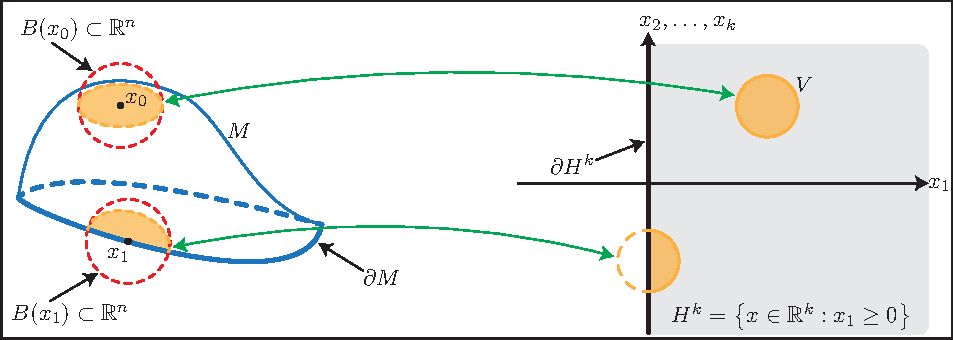
\includegraphics[width=0.99\textwidth]{figures/ch9/5bndry_mfd_def.pdf}
		\caption{An illustration of the manifold with boundary $M$ and a parameterization mapping its boundary to $\partial H^{k}$.}
		\label{fig:bndry_mfd_def}
	\end{figure}
\end{definition}

Closed intervals, closed cyclinders, and closed hollow spheres are all manifolds with boundaries, however it is not always the case that simply taking the closure of a manifold yields a manifold with boundary. For instance the interior of a rectangle is a manifold (using the identity as a parameterization), however as the corners are not smooth the closure is not a manifold.

\begin{definition}
	Given a $k$-dimensional manifold $M\subset \mathbb{R}^{n}$ with the local parameterization at $x$ given by $\Phi:: U\subset \mathbb{R}^k \to V\subset M \subset \mathbb{R}^n$ (assume for simplicity that $\Phi(0)=x\in V$), the \emph{tangent space of the manifold} is then defined as
	\begin{align}
		\boxed{
			T_{x}M= \textrm{Range} [D\Phi(0)].
		}
	\end{align}
	The intuition as to why this is called the tangent space is show in Fig. \ref{fig:tangent_space_def}.
	\begin{figure}[h!]
		\centering
		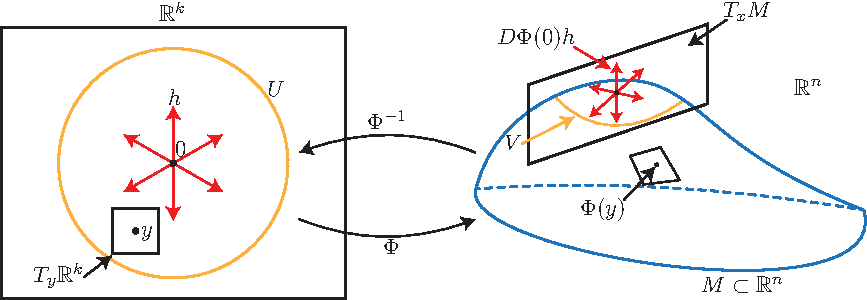
\includegraphics[width=0.99\textwidth]{figures/ch9/6tangent_space_def.pdf}
		\caption{The tangent space of a manifold $M$. The map $D\Phi(0)$ maps the left image to the plane indicated in the right image.}
		\label{fig:tangent_space_def}
	\end{figure}
\end{definition}

Note here how the differential is defined
\begin{align}
	D \Phi(x)h = \lim_{s \to 0} \frac{\Phi(x + sh) - \Phi(x)}{s}.
\end{align}
Therefore the map $D\Phi(y)$ is a map from the tangent space of $\mathbb{R}^{k}$ at $y$ to the tangent space of $M$ at $\Phi(y)$, i.e. $D\Phi(y): T_{y}\mathbb{R}^{k}\to T_{\Phi(y)}M$. 

\begin{remark}[]
	Note a few facts about tangent spaces:
	\begin{enumerate}
		\item Although it appears that $T_{x}M$ depends on the parameterization $\Phi$, it actually does not;
		\item The dimension of the tangent space, which is well defined as it is a linear subspace of $\mathbb{R}^{n}$, is equal to the dimension of $M$, namely $k$;
		\item A map $f:M\to N$ between manifolds induces a linear mapping between the appropriate tangent spaces of the manifolds. Denoting by $\Phi$ and $\Psi$ the respective local parameterizations, the induced map between parameter spaces is $F= \Psi^{-1} \circ f \circ \Phi$. This is a mapping between linear spaces and $DF$ is well-defined. In turn, this implies that $Df$ is well-defined and by the chain rule is equal to $D\Psi \circ DF \circ D\Phi^{-1}$, therefore it is possible to differentiate mappings between manifolds. Then we have the sought-after mapping between tangent spaces 
			\begin{align}
				Df: T_{x}M \to T_{f(x)}N.
			\end{align}
			These maps are illustrated in Fig. \ref{fig:induced_tangent_map}.
			\begin{figure}[h!]
				\centering
				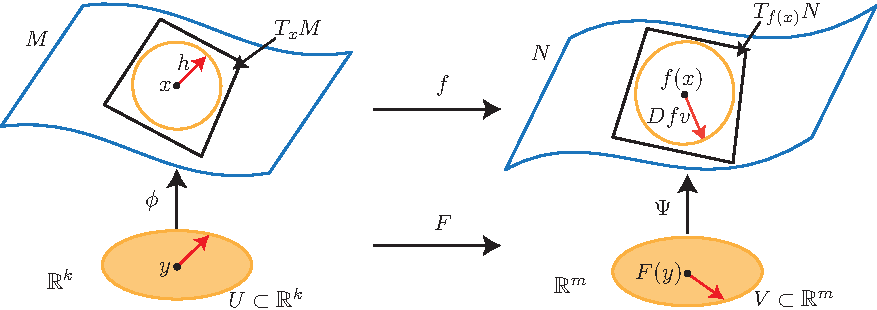
\includegraphics[width=0.99\textwidth]{figures/ch9/7induced_tangent_map.pdf}
				\caption{The commutative diagram along with the respective spaces illustrated for the induced map between tangent spaces.}
				\label{fig:induced_tangent_map}
			\end{figure}
	\end{enumerate}
\end{remark}

\begin{definition}
	The set of all tangent spaces, labelled by their base points is called the \emph{tangent bundle}
	\begin{align}
		\boxed{
			TM = \left\{ (x,v):\ x\in M,\ v\in T_{x}M \right\} = \bigcup_{x\in M}(x, T_{x}M).
		}
	\end{align}
The tangent bundle is a $2k$-dimensional manifold.	
\end{definition}

By labelling tangent vectors with their respective base points, different tangent spaces are separate \emph{fibers} of the tangent bundle. In general $TM \neq M \times \mathbb{R}^{k}$, i.e. the tangent bundle is not a global direct product. In fact, locally, each tangent bundle is trivial (the direct product), this just does not extend globally. However, for $M=\mathcal{S}^{2}$ the tangent bundle is diffeomorphic to $\mathcal{S}^{2} \times \mathbb{R}^{2}$. 

\begin{definition}
	The \emph{normal space}, unlike the tangent space, depends on the ambient space. For a $k$-dimensional manifold $M$ embedded in $\mathbb{R}^{n}$, the normal space at a point $x$, $N_{x}M$, is the orthogonal complement of the tangent space. For their direct sum it holds, that 
	\begin{align}
		\boxed{
			T_{x}M \oplus N_{x}M = T_{x}\mathbb{R}^{n}.
		}
	\end{align}
	Therefore, the dimensional of the normal space is $n-k$. The normal space is drawn in Fig. \ref{fig:normal_space_def}.	
	\begin{figure}[h!]
		\centering
		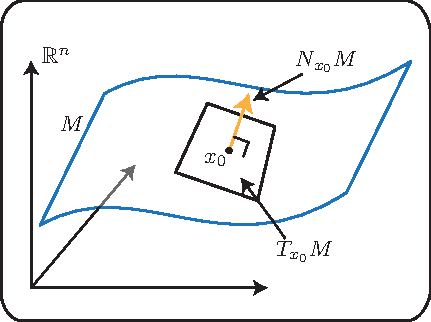
\includegraphics[width=0.6\textwidth]{figures/ch9/8normal_space_def.pdf}
		\caption{The normal space of a manifold $M$ at the point $x_0$ along with the tangent space at the same point.}
		\label{fig:normal_space_def}
	\end{figure}
\end{definition}

\begin{definition}
	Analog to the tangent bundle, the \emph{normal bundle} is the collection of normal spaces of the manifold $M$ labelled by their base points
	\begin{align}
	\boxed{
		NM = \left\{ (x,v):\ x\in M,\ v\in N_{x}M \right\}.
	}
	\end{align}
\end{definition}
By labelling normal vectors with their base points, intersections are avoided as shown in Fig. \ref{fig:normal_vector_intersection}.
\begin{figure}[h!]
	\centering
	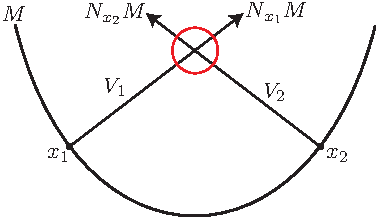
\includegraphics[width=0.6\textwidth]{figures/ch9/9normal_vector_intersection.pdf}
	\caption{Intersecting normal vectors, these are avoided by labelling vectors with their base points.}
	\label{fig:normal_vector_intersection}
\end{figure}

\begin{definition}
	A \emph{subbundle} of the normal bundle is any $x$-dependent family of subspaces of $N_{x}M$, which is smooth in $x$.
\end{definition}
An example of such a subbundle is given in Fig. \ref{fig:subbundle_ex}, where the smooth family of subspaces is given by $S(x)\subset N_{x}M$.
\begin{figure}[h!]
	\centering
	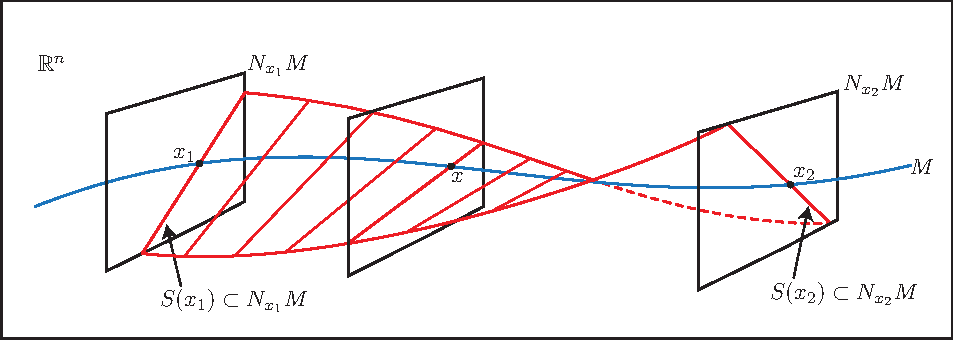
\includegraphics[width=0.99\textwidth]{figures/ch9/10subbundle_ex.pdf}
	\caption{A subbundle of the manifold $M$, each base point $x\in M$ is a base point of $S(x)$, a fiber of the normal bundle.}
	\label{fig:subbundle_ex}
\end{figure}

\newpage
\section{Theory of normally hyperbolic invariant manifolds}
The starting point for the following section will be of an autonomous dynamical system
\begin{align}
	\dot{x}=f(x);\quad x \in \mathbb{R}^{n};\quad f\in\mathcal{C}^{r}\ r\geq 1.
\end{align}
Furthermore, let $M_0\subset \mathbb{R}^{n}$ be a $k$-dimensional, compact, $\mathcal{C}^{1}$-manifold with boundary $\partial M_{0}$.

\begin{definition}
	The manifold $M_0$ is an \emph{overflowing invariant manifold} if $f(x)$ points strictly outwards of $\partial M_0$. A special case of this is when $\partial M_0= \emptyset$.
\end{definition}

There are three central questions for what happens to this manifold which we will address:
\begin{enumerate}
	\item Does it persists (survive smoothly)?
	\item Is it stable (what happens to nearby trajectories)?
	\item What is the interior structure of the stable/unstable manifolds of $M_0$?
\end{enumerate}

\begin{ex}[]
	Consider the system
	\begin{align}
		\begin{dcases}
			\dot{x}= -x(1-x)(1+x) \\
			\dot{y} = \alpha y
		\end{dcases}
		;\quad 0 < \alpha \leq 1.
	\end{align}
	Now define $M_0$ to be the closed interval $[-1-\varepsilon, 1 + \varepsilon]\times \{0\}$. This manifold is of dimension 1, has nonempty boundary $\{-1-\varepsilon, 1+\varepsilon\}$, is compact, and smooth. At each point in the boundary, $f$ is pointing away from $M_0$. Therefore, $M_0$ is an overflowing invariant manifold. We also have that $W^{S}_{ \textrm{loc}}(M_0)$ is nonempty, meanwhile $W^{U}_{ \textrm{loc} }(M_0)$ is empty. Trajectories of this dynamical system along with $M_0$ and the stable local manifold are depicted in Fig. \ref{fig:overflowing_mfd_ex1}.
	\begin{figure}[h!]
		\centering
		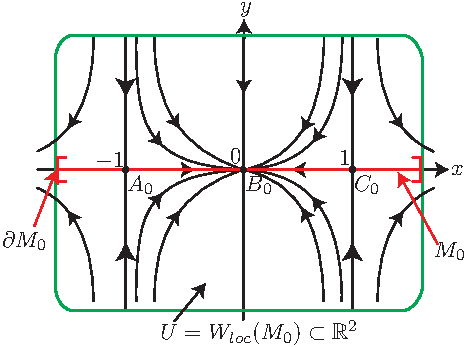
\includegraphics[width=0.6\textwidth]{figures/ch9/11overflowing_mfd_ex1.pdf}
		\caption{An illustration of the trajectories of the dynamical system, the overflowing invariant manifold $M_0$, its boundary, and the local stable manifold drawn in green. The fixed points $A_0$, $B_0$, and $C_0$ are also shown.}
		\label{fig:overflowing_mfd_ex1}
	\end{figure}

	Now we may ask if $M_0$ is robust under perturbations (if it persists). For example under the perturbation
	\begin{align}
		\begin{dcases}
			\dot{x} = -x(1-x)(1+x) -\varepsilon y \\
			\dot{y} = - \alpha y + \varepsilon x
		\end{dcases}
		;\quad 0 \leq \varepsilon \ll 1.
	\end{align}
	The fixed points $A_0=(-1,0)$, $B_0=(0,0)$, and $C_0=(1,0)$ are hyperbolic, therefore they persist. In fact $B_0$ does not move at all. The other fixed points move to new perturbed counterparts, i.e. $A_0,C_0 \to A_{\varepsilon}, C_{\varepsilon}$. From the second equation, we see that the y coordinate of the perturbed fixed point becomes $y_\varepsilon= \varepsilon/\alpha x_\varepsilon$. That is, $C_\varepsilon$ moves upwards and $A_\varepsilon$ moves downwards.

	At $B_0 = B_{\varepsilon}$ we can linearize to find
	\begin{align}
		\begin{pmatrix}
			\dot{x} \\ \dot{y}
		\end{pmatrix}
		 = 
		 \begin{pmatrix}
			 -1 & - \varepsilon \\
			 \varepsilon & -\alpha 
		 \end{pmatrix}
		 \begin{pmatrix}
		 	x \\ y
		 \end{pmatrix}
		. 
	\end{align}
Depending on $\alpha $ we differentiate two cases.
\begin{enumerate}
	\item $\bm{\alpha =1} $ In this case the eigenvalues split in a vertical fashion, as shown in Fig. \ref{fig:eigv_vertical_split}. The stable node turns into a stable spiral, which, when connected to the perturbed fixed points $A_{\varepsilon}$ and $C_{\varepsilon}$ cannot be diffeomorphic to $M_0$.
		\begin{figure}[h!]
			\centering
			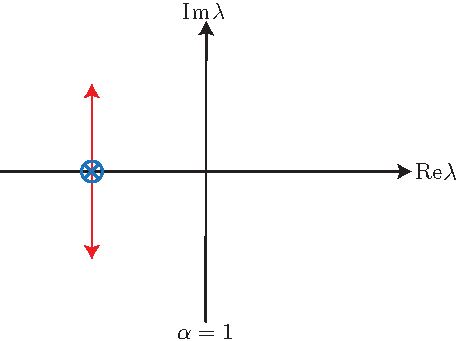
\includegraphics[width=0.6\textwidth]{figures/ch9/11_5vertical_split.pdf}
			\caption{The eigenvalues splitting in a vertical fashion for $\alpha=1$.}
			\label{fig:eigv_vertical_split}
		\end{figure}
	\item $\bm{0<\alpha<1}$ The eigenvalues remain real, but the manifold $M_0$ does not persist smoothly. To show this, consider a perturbation of the form
		\begin{align}
		\begin{dcases}
			\dot{x} = -x(1-x)(1+x) -\varepsilon y \\
			\dot{y} = - \alpha y + \varepsilon x^2
		\end{dcases}
		;\quad 0 \leq \varepsilon \ll 1.
	\end{align}The perturbation in the $\dot{y}$-equation, $\varepsilon x^2$, causes the perturbed fixed points $A_\varepsilon$ and $C_\varepsilon$ to move upwards, since their $y-$coordinates are $y_\varepsilon  = \frac{\varepsilon}{\alpha}x_\varepsilon^2$. The perturbed curve connecting $A_\varepsilon$, $B_\varepsilon$ and $C_\varepsilon$ has a cusp at $B_\varepsilon$ and cannot be diffeomorphic to $M_0$.
\end{enumerate}
Thus in each case, no smooth transformation to $M_0$ exists and therefore there is no persistence. The perturbed geometries are shown in Fig. \ref{fig:nondiffeo_pertubation}.
\begin{figure}[h!]
	\centering
	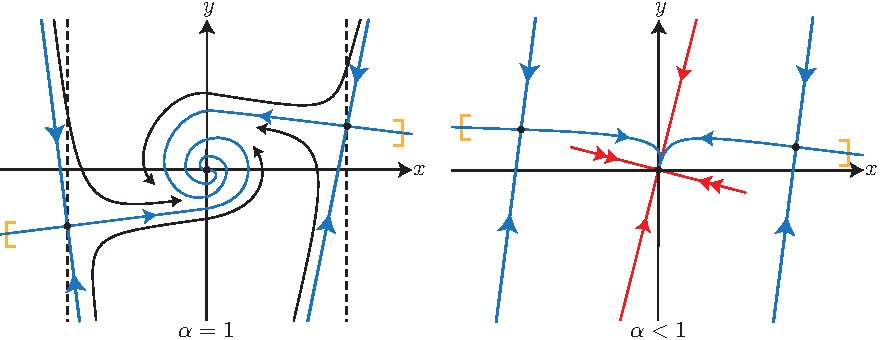
\includegraphics[width=0.99\textwidth]{figures/ch9/11_75alpha_perturbation.pdf}
	%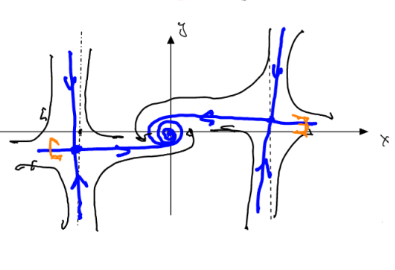
\includegraphics[width=0.4\textwidth]{figures/ch9/11_75alpha_one_perturb.png}
	%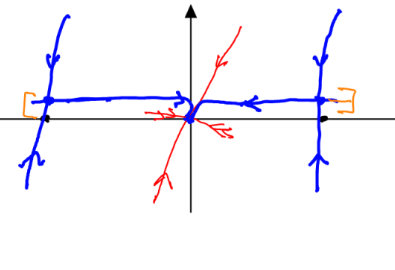
\includegraphics[width=0.4\textwidth]{figures/ch9/11_75alpha_small_perturb.png}
	\caption{Left: The geometry for $\alpha=1$. Right: The geometry for $\alpha<1$.}
	\label{fig:nondiffeo_pertubation}
\end{figure}

\end{ex}

The reason for the destruction of the manifold here was the normal rate of attraction being less than or equal to the tangential rate of attraction at one point. This can be exemplified as follows.

\begin{ex}[]
	Consider the dynamical system
	\begin{align}
		\begin{dcases}
			\dot{x} = -x(1-x)(1+x) + \varepsilon y \\
			\dot{y} = - \frac{3}{2} y - \varepsilon x
		\end{dcases}
.		
	\end{align}
	This is the specification of the previous example to $\alpha = \frac{3}{2}$. If we linearize at the point $B_0$ for $\varepsilon = 0 $ we find
	\begin{align}
	\begin{dcases}
		\dot{x} = - x \\
		\dot{y} = -\frac{3}{2} y
	\end{dcases}
	.	
	\end{align}
	The solution to the linearized system is
	\begin{align}
		\begin{dcases}
			x(t) = x_0 e^{-t} = x_0 \left(e^{-1} \right)^{t} \\
			y(t) = y_0 e^{-\frac{3}{2}t} = y_0 \left(e^{-\frac{3}{2}}\right)^{t}
		\end{dcases}
		\implies y = y_0 \left(\frac{x}{x_0}\right)^{\frac{3}{2}}. \label{eq9:914}
	\end{align}
	The eigenvalue constellation and linearized phase portrait, along with the implied nonlinear phase portrait for this system are show in Fig. \ref{fig:alpha_specification}. From \eqref{eq9:914} we see that the phase curves of the system are only $\mathcal{C}^1$ because of the power of $\frac{3}{2}$. In the nonlinear system, this implies that the perturbed manifold $M_\varepsilon$ exists, but is also only $\mathcal{C}^1$-smooth. Thus, the ratio between normal and tangential contraction determines the smoothness of $M_\varepsilon$.
	\begin{figure}[h!]
		\centering
		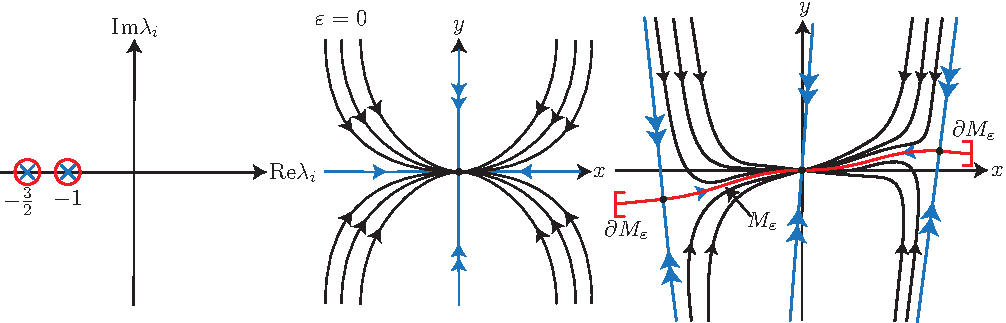
\includegraphics[width=0.99\textwidth]{figures/ch9/12alpha_specification.pdf}
%		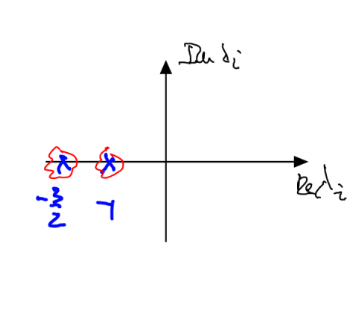
\includegraphics[width=0.27\textwidth]{figures/ch9/12alpha_specification_1.pdf}
%		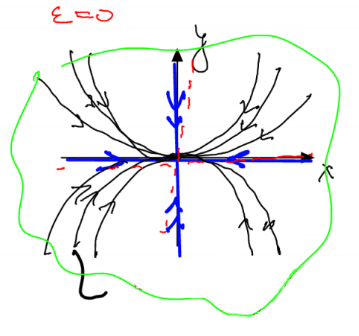
\includegraphics[width=0.27\textwidth]{figures/ch9/12alpha_specification_2.png}
%		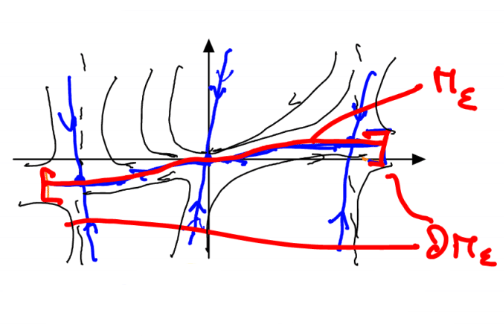
\includegraphics[width=0.4\textwidth]{figures/ch9/12alpha_specification_3.png}
		\caption{Left: The eigenvalue constellation for the linearization around $B_0$ for $\varepsilon=0$. Middle: The linearized phase portrait around $B_0$. Right: The nonlinear phase portrait with the nearby overflowing invariant manifold $M_{\varepsilon}$.}
		\label{fig:alpha_specification}
	\end{figure}

	One can check here that $\dot{y}= (r+\mu )y + \varepsilon x$ would give $\mathcal{C}^{r}$ differentiability for $M_{\varepsilon}$ for $0 \leq \mu \ll 1$. Formally, for $\mu=0 $ we would have $\mathcal{C}^{\infty }$ differentiability, but only for the linear part, and this would not be robust.	
\end{ex}

The general challenge is to quantify the growth/contraction rates in the normal and tangential directions, i.e. how do we determine the rates away from fixed points along trajectories.

Recall our setup with the compact, overflowing invariant $\mathcal{C}^{r}$ manifold $M_0 \subset   \mathbb{R}^{n}$ of dimension $k$, for $r\geq 1$ and the dynamical system 
\begin{align}
	\dot{x} = f(x);\quad x \in \mathbb{R}^{n};\quad f\in \mathcal{C}^{r}.
\end{align}
Now consider the \emph{inverse linearized flow map} on the tangent bundle of $\mathbb{R}^{n}$ for some $t\geq 0$
\begin{align}
	(F^{-t}, DF^{-t}):\ T\mathbb{R}^{n} \to T\mathbb{R}^{n};\ (p,v) \mapsto \left(F^{-t}(p), DF^{-t}(p)v\right).
\end{align}
This map is depicted in Fig. \ref{fig:inv_lin_flow_map}.
\begin{figure}[h!]
	\centering
	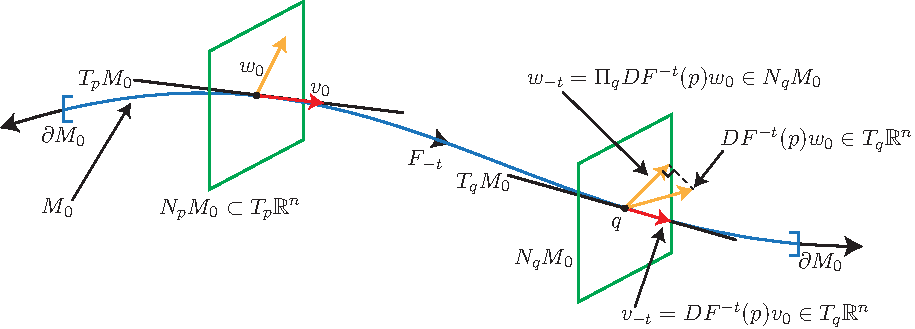
\includegraphics[width=0.99\textwidth]{figures/ch9/13inv_lin_flow_map.pdf}
	\caption{The inverse linearized flow map. We have $q=F^{-t}(p)\in M_0$ and the red arrow on the right is $v_{-t}=DF^{-t}(p)v_0 \in T_{q}M_0$ for $v_0 \in T_{p}M_0$. The map $\Pi_{q}$ is the orthogonal projection onto $N_{q}M_0$.}
	\label{fig:inv_lin_flow_map}
\end{figure}

To quantify the rate of normal attraction we define for $w_0 \in N_{p}M_0$, as in Fig. \ref{fig:inv_lin_flow_map}, $w_{-t}\in N_{q}M_0$ to be $\Pi_{q}DF^{-t}(p)w_0 $. If we have repulsion in backward time, $\| w_{-t}\| \gg \| w_0\|$, with an exponential rate, i.e. 
\begin{align}
	\frac{\|w_0 \|}{\| w_{-t}\|}\sim e^{-\alpha t}	= (e^{-\alpha })^{t}; \quad \alpha >0; \quad t \to \infty ,
\end{align}
then the best estimate for such an $e^{-\alpha }$ is 
\begin{align}
	\boxed{
		\nu(p) = \inf \left\{ a \in \mathbb{R}^{+}:\ \lim_{t\to\infty }{\frac{\|w_0\|}{\|w_{-t}\|}}/{a^{t}} = 0,\ \forall w_0 \in N_{p}M_0 \right\}.
	}
\end{align}
The $\inf $ is defined as the largest lower bound. The idea behind this, is that for large $a$, the quotient will go to zero, if we start to lower $a$ until this trend changes. We then pick the largest lower bound for this change.

If $e^{-\alpha }=a \sim \nu(p) < 1$ then $M_0$ is exponentially attracting in backward time. Note that the orbit from $p$ will generally not approach a fixed point. Furthermore, $\log(\nu(p))$ will generally not be the eigenvalue of a Jacobian (the linearized flow map at a fixed point).

Next, we would like to quantify the relationship between the normal and tangential rates. If we have
\begin{align}
{\frac{\| w_0 \|}{\|w_{-t}\|}}/{\frac{\|v_0\|}{\|v_{-t}\|}} \sim \frac{e^{-\alpha t}}{e^{-\alpha t \cdot \frac{1}{\rho}}}
\end{align}
for some $\rho \in \mathbb{R}$ and $\alpha >0$ as $t\to \infty $ then define for the best asymptotic estimate for $1/\rho$, define $\sigma(p)$ to be
\begin{align}
	\boxed{
		\sigma(p) = \inf \left\{ b \in \mathbb{R}:\ \lim_{t\to \infty }\left({\frac{\|w_0\|}{\|w_{-t}\|}} \right) ^{b} /{\frac{\|v_0\|}{\|v_{-t}\|}} = 0,\ \forall w_0 \in N_{p}M_0,\ \forall v_0 \in T_{p}M_0 \right\}.
	}
\end{align}
The numbers $\nu(p)$ and $\sigma(p)$ are called {\emph Fenichel-type numbers}. They are sometimes also referred to as Lyapunov-type numbers or sometimes simply Type-numbers. If $\sigma(p) \sim \frac{1}{\rho} < \frac{1}{s}$ for some $s\in \mathbb{Z}^{+}$, then the normal decay to $M_0$ is $s$-times stronger than the tangential compression along $M_0$, at least along the trajectory through $p$.

\begin{remark}[Properties of Fenichel-type numbers]
 First, each are constant along trajectories, and dependent only on the $\alpha $-limit set of the trajectory (the set of limit points as $t \to -\infty $). Also, both $\sigma(p)$ and $\nu(p) $ are upper-semicontinuous in $p$ ($\limsup_{p \to p_0} \sigma(p) \leq \sigma(p_0)$).
\end{remark}

to discuss the computation of the Fenichel-type numbers. To this end, define two functions
\begin{align}
	A_{t}(p) &= \left. DF^{-t}(p) \right|_{T_{p}M_0}:\ T_{p}M_0 \to T_{q}M_0;\ q = F^{-t}(p); \\
	B_{t}(p) &= \left. \Pi_{p}DF^{t}(F^{-t}(p)) \right|_{N_{F^{-t}(p)}M_0}:\ N_{F^{-t}(p)}M_0 \to N_{p}M_0.
\end{align}
The reason for the $F^{-t}(p)$ being the inner argument for $B_{t}$ is that we need to step back in order to safely evaluate the linearized map in forward time. With these functions in hand we can calculate the Fenichel-type numbers equipped with the next theorem.

\begin{theorem}[Fenichel (1971)]
We have that the following holds
\begin{align}
	\boxed{\nu(p) = \limsup_{t\to \infty }\| B_{t}(p)\|^{\frac{1}{t}}; }
\end{align}
and if $\nu(p)<1$, then
\begin{align}
	\boxed{\sigma(p) = \limsup_{t\to \infty }\frac{\log\left( \| A_{t}(p) \| \right)}{-\log \left( \| B_{t}(p) \| \right)}.}
\end{align}
\end{theorem}

\begin{ex}[]
	Consider the dynamical system
	\begin{align}
		\begin{dcases}
			\dot{x} = -x(1-x)(1+x) \\
			\dot{y} = -by
		\end{dcases}
		;\quad b>0.
	\end{align}
	Further, define $M_0 = \left\{ (x,y):\ x\in \left[ -\frac{3}{2}, \frac{3}{2}\right],\ y=0 \right\}$. Using the previous theorem, it is possible to show
	\begin{align}
		\nu (A_0) = \nu (C_0) = e^{-b}; \quad \sigma(A_0) = \sigma(C_0) = - \frac{2}{b}; \quad
		\nu (B_0) = e^{-b}; \quad \sigma(B_0) = \frac{1}{b}.
	\end{align}
	The points $A_0$, $B_0$, and $C_0$ along with the manifold $M_0$ are illustrated in the phase space in Fig. \ref{fig:fenichel_ex1}.
	\begin{figure}[h!]
		\centering
		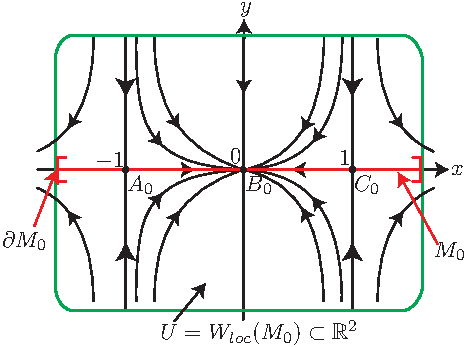
\includegraphics[width=0.6\textwidth]{figures/ch9/14fenichel_ex1.pdf}
		\caption{$A_0$, $B_0$, and $C_0$ along with the manifold $M_0$ are illustrated in the phase space.}
		\label{fig:fenichel_ex1}
	\end{figure}
\end{ex}

\begin{definition}
	The manifold $M_0$ is an \emph{$r$-normally hyperbolic invariant manifold} (NHIM) if
	\begin{enumerate}
		\item $\nu (p)<1$ for all $p\in M_0$ ;
		\item $\sigma(p) < \frac{1}{r}$ for all $p \in M_0$.
	\end{enumerate}	
\end{definition}
\begin{remark}[]
	If there is no tangential compression, then $\sigma(p)<0$ and $(ii)$ holds automatically for all $r$.
\end{remark}

Building on the previous results, we have the next the next result.
\begin{theorem}[Fenichel (1971)]
Assume we have
\begin{align}
	\dot{x}= f_{ \textrm{pert} }(x) = f_{0}(x) + \Delta f(x);\quad f_0, \Delta f \in \mathcal{C}^{r},\ r\geq 1,
\end{align}
for a compact, overflowing invariant (under $f_0(x)$) manifold $M_0$ which is $\mathcal{C}^{r}$ and $r$-normally hyperbolic. Then for $\|\Delta f \|_{\mathcal{C}^{1}}$ small enough, there exists an overflowing invariant manifold $\tilde{M}_0$ for $\dot{x}=f_{ \textrm{pert} }(x)$, such that
\begin{enumerate}
	\item $\tilde{M}_{0}$ is $\mathcal{C}^{1}$-close to $M_0$ and $\mathcal{C}^{r}$-diffeomorphic to $M_0$ ;
	\item All close enough trajectories converge to $\tilde{M}_{0}$ as $t \to \infty $, as long as they stay in a neighborhood of $\tilde{M}_{0}$.
\end{enumerate}
This result is depicted in Fig. \ref{fig:fenichel_thm2}.
\begin{figure}[h!]
	\centering
	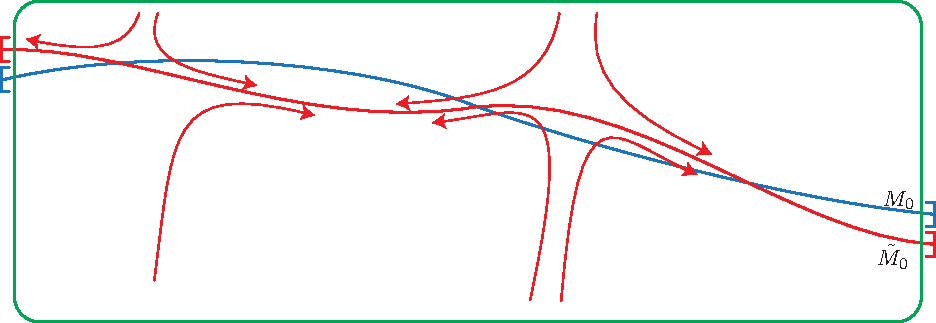
\includegraphics[width=0.99\textwidth]{figures/ch9/15fenichel_thm2.pdf}
	\caption{The manifolds $M_0$ and $\tilde{M}_{0}$ illustrated within the locally invariant manifold $W^{S}_{ \textrm{loc} }(\tilde{M}_{0})$ (green).}
	\label{fig:fenichel_thm2}
\end{figure}
\end{theorem}

\begin{remark}[]
	The following hold:
	\begin{enumerate}
		\item If $M_0$ is compact, normally hyperbolic invariant (without boundary), then it attracts \underline{all} nearby trajectories ($M_0$ is an attractor that smoothly persists);
		\item The integer $r$ featured in the theorem is the minimum of the integers $r_i\in \mathbb{Z}^{+}$, where $f \in \mathcal{C}^{r_1}$, $M_0 \in \mathcal{C}^{r_2}$, and $\sigma(p) < \frac{1}{r_3}$;
		\item Similar results hold for inflowing invariant manifolds that repel nearby initial conditions ($M_0$ and $\tilde{M}_{0}$ are persistent repellers);
		\item The theory also extends to saddle-type invariant manifolds too, e.g. the unstable manifold of an overflowing invariant manifold. In this case assume that the tangent bundle $\left.T\mathbb{R}^{n}\right|_{M_0}$ has an invariant splitting, i.e. $T_{p}\mathbb{R}^{n} = T_pM_0 \oplus N_{p}^{U}M_0 \oplus N_{p}^{S}M_0$, then there exists an additional Fenichel-type number for $N^{U}M_0$ and $W^{U}_{ \textrm{loc} (M_0)}$ is robust. This is shown in Fig. \ref{fig:fenichel_thm_rmks}.
		\begin{figure}[h!]
			\centering
			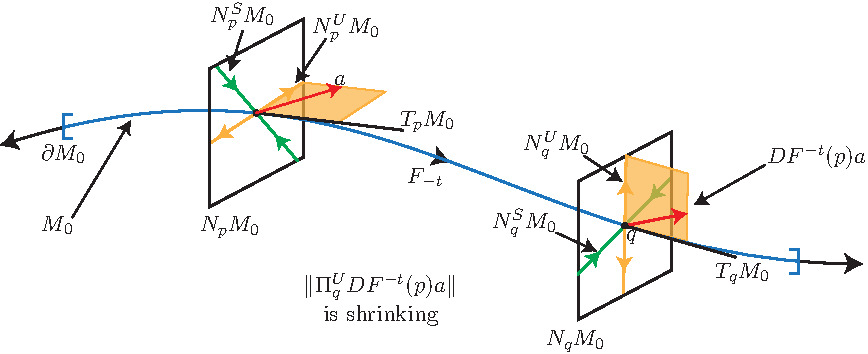
\includegraphics[width=0.99\textwidth]{figures/ch9/16fenichel_thm_rmks.pdf}
			\caption{The effect of the tangent bundle having an invariant splitting with the addition of a Fenichel-type number for $N^{U}M_0$ and robust $W^{U}_{ \textrm{loc} }(M_0)$.}
			\label{fig:fenichel_thm_rmks}
		\end{figure}
	\end{enumerate}
\end{remark}
For more see \cite{Wiggins1994}.

\section{Geometric singular perturbation theory}
Singular perturbation theory is the study of systems with two different time scales, i.e. of the form
\begin{align}
	\begin{dcases}
		\dot{x} &= f(x,y,\varepsilon) \\
		\varepsilon \dot{y} &= g(x,y,\varepsilon)
	\end{dcases}
	;\quad 0 \leq \varepsilon \ll 1; \quad f,g \in \mathcal{C}^{1}. \label{eq9:spt_1}
\end{align}
In such systems $x \in \mathbb{R}^{n}$ is called the \emph{slow variable} and $y \in \mathbb{R}^{m}$ is the \emph{fast variable}.
\begin{ex}[One degree of freedom mechanical oscillator with a small mass]
	An example of a system with two different time scales is a single degree of freedom mechanical oscillator with a small mass, the dynamical system is given by
	\begin{align}
		\varepsilon \ddot{x} + F(x, \dot{x}, \varepsilon) = 0 \implies
		\begin{dcases}
			\dot{x} &=y \\
			\varepsilon \dot{y} &= - F(x,y, \varepsilon)
		\end{dcases}
		.
	\end{align}
	Note that $\dot{y} = \frac{1}{ \varepsilon}F(x,y,\varepsilon)$ implies that $y$ changes very quickly. The equations for $\dot{y}$ become singular as $\varepsilon \to 0$, hence we have singular perturbation (the smooth dependence of solutions on $\varepsilon$ does not apply).
\end{ex}

The classical approach to such systems is to set $\varepsilon =0 $ in \eqref{eq9:spt_1}, obtaining
\begin{align}
	\begin{dcases}
		\dot{x} = f(x,y, 0) \\
		0 = g(x,y,0)
	\end{dcases}
	.
\end{align}
This is a mixed differential-algebraic system of equations. We solve $g (x,y,0)=0$ for $y=G_{0}(x)$, expand in $\varepsilon$, and plug this into $\dot{x}=f(x,y,\varepsilon)$. Sometimes this works, however this is not guaranteed. Instead we will follow \cite{Fenichel1979}.

First, turn this into a regular perturbation problem by introducing the fast time $t = \varepsilon \tau$, i.e $\tau = \frac{t}{\varepsilon}$ for $0 < \varepsilon \ll 1$. This change of coordinates induces via the chain rule the Jacobian
\begin{align}
	\frac{d (\cdot) }{dt} = \frac{d( \cdot) }{d \tau }\frac{d \tau}{dt}.
\end{align}
The differential of a function $f$ with respect to $t$ will be denoted by $\dot{f}$, and is equal to $f' \frac{1}{\varepsilon}$, with $f'$ denoting the differential of $f$ with respect to $\tau$. Hence we obtain the rescaled system
\begin{align}
\begin{dcases}
	x' = \varepsilon f(x,y, \varepsilon) \\
	y' = g(x,y, \varepsilon)
\end{dcases}
. \label{eq9:spt_2}	
\end{align}
Note that \eqref{eq9:spt_2} is a regular perturbation problem from a \underline{fictitious limit}. The systems \eqref{eq9:spt_1} and \eqref{eq9:spt_2} are not equivalent for  $\varepsilon=0$, but are equivalent for any $\varepsilon >0$. 

We analyze the $\varepsilon=0$ limit next, i.e.
\begin{align}
	\begin{dcases}
		x' = 0 \\
		y' = g(x,y,0)
	\end{dcases}
	.\label{eq9:spt_3}
\end{align}
Assume that that there exists a pair $(x_0, y_0)$ such that $g(x_0, y_0,0)=0$, i.e. a fixed point of \eqref{eq9:spt_3}. Then we have $m$ equations for $m$ unknowns $y_0$, by the Implicit Function Theorem a unique nearby zero $y = \varphi_0(x)$ with $\varphi \in \mathcal{C}^{1}$ exists whenever we have that the following hold
\begin{enumerate}
	\item The matrix $D_{y}g(x_0, y_0, 0)$ is nonsingular;
	\item The derivative $D_{x}g(x_0, y_0, 0)$ exists near $(x_0, y_0)$.
\end{enumerate}
In which case we can define the $n$-dimensional invariant manifold filled with fixed points 
\begin{align}
\boxed{
M_0 = \left\{ (x,y):\ y= \varphi_0(x),\ x\in U,\ U  \textrm{ compact},\ \det\left[D_{y}g(x,y,0)\right]\neq 0 \right\} .
}
\end{align}
This manifold is called the \emph{critical manifold} and an example is shown in Fig. \ref{fig:critical_mfd_def}.
\begin{figure}[h!]
	\centering
	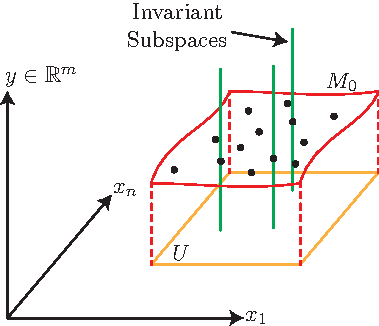
\includegraphics[width=0.55\textwidth]{figures/ch9/17crit_mfd_def.pdf}
	\caption{An example of the critical manifold $M_0$ (red) filled with fixed points, an $n$-dimensional invariant subspace (green line) passes through each fixed point.}
	\label{fig:critical_mfd_def}
\end{figure}

Next, we linearize. Begin by defining $\eta = y - \varphi_0(x)$, then calculate the derivative of $\eta $ with respect to $\tau$ 
\begin{align}
	\eta' = y' - \underbrace{\varphi_0' x'}_{=0} = g(x, \varphi_0(x) + \eta, 0) = \underbrace{g(x, \varphi_0(x), 0) }_{=0} + D_{y}g(x, \varphi_0(x), 0) \eta + \mathcal{O}(\eta^2).
\end{align}
Thus our linearization is $\eta' = D_{y} g(x, \varphi_0(x), 0 ) \eta$, due to the nonsingularity condition before we know that $\lambda_{i}(D_{y}g(x,y,0)) \neq 0$ for $i=1,\ldots, m$. If, in addition, we have that $ \textrm{Re}[\lambda_i(D_{y}g(x,y,0)]\neq 0  $ for $i = 1, \ldots, m$, then $M_0$ is normally hyperbolic.

The most important case is when $M_0$ is normally attracting, i.e. when \newline $ \textrm{Re} [\lambda_i(D_{y}g(x,y,0) ] < 0$ for each $i=1,\ldots, m$.  In which case $M_0$ is $r$-normally hyperbolic, where if $\varphi_0(x)$ is $\mathcal{C}^{r}$ for any $r\in \mathbb{Z}^{+}$ then $M_0$ persists for $\varepsilon$ small enough. 

The classical formal approach often fails when there exist eigenvalues with positive real parts, i.e. when $M_0$ is unstable.

For $\varepsilon>0$ and with eigenvalues of only strictly negative real parts (as before), we get the perturbation $M_\varepsilon$ of $M_0$. This perturbed manifold is the \emph{slow manifold}, motion on it is of $\mathcal{O}(\varepsilon)$ speed, and in this case it is attracting. We have that for the $\mathcal{C}^{1}$ function $\varphi_{\varepsilon}$ (also in $\varepsilon$ as long as $g(x,y,\varepsilon)$ is $\mathcal{C}^{1}$ in $\varepsilon$)
\begin{align}
	y = \varphi_{\varepsilon}= \varphi_0(x) + \varepsilon \varphi_1(x) + \mathcal{O}(\varepsilon^{2}).
\end{align}
Thus $y$ is a smooth graph over the domain $U$. The perturbed manifold and the representation of $y$ as a smooth graph over $U$ is shown in Fig. \ref{fig:singular_perturbed_mfd}.
\begin{figure}[h!]
	\centering
	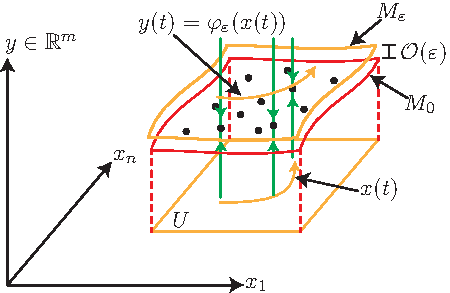
\includegraphics[width=0.6\textwidth]{figures/ch9/18singular_pert_mfd.pdf}
	\caption{The perturbed manifold $M_{\varepsilon}$ near the critical manifold $M_0$ as well as the representation of $y$ as a smooth graph over the domain $U$.}
	\label{fig:singular_perturbed_mfd}
\end{figure}

We can reduce to the slow manifold and find the reduced flow
\begin{align}
	\left. x' \right|_{M_{\varepsilon}} &= \varepsilon\left. f(x,y, \varepsilon)\right|_{M_{\varepsilon }}	= \varepsilon f(x, \varphi_\varepsilon(x), \varepsilon) \\
					    &= \varepsilon \left[ f(x, \varphi_0 (x) , 0) + \varepsilon\left( D_{\varepsilon} f(x, \varphi_0(x), 0) + D_{y}f(x, \varphi_0 (x), 0) \varphi_1(x) \right) \right] + \mathcal{O}(\varepsilon ^{3}).
\end{align}
In the original time $t$ we find the \emph{reduced flow}
\begin{align}
	\boxed{
		\dot{x} = f(x, \varphi_0(x), 0) + \varepsilon \left[ D_{\varepsilon}f(x, \varphi_0(x), 0) + D_{y} f(x, \varphi_0(x), 0) \varphi_1(x) \right] + \mathcal{O}(\varepsilon^{2}).
	}
\end{align}
The leading order restricted flow on the attractor $M_{\varepsilon}$ is given by $\dot{x} = f(x, \varphi_0(x), 0)$. Any structurally stable feature of this leading-order reduced flow will persist on the attractor. For other features, we need higher-order terms. The dynamics near the slow manifold is attractive towards $M_{\varepsilon}$ if $ \textrm{Re} [\lambda_i ( D_{y}g(x,y,0)]<0$ for $i=1, \ldots, m$ for all $(x,y) \in M_0$, i.e. $W^{U}_{ \textrm{loc} }(M_{\varepsilon})$ is empty. Furthermore, we get the stable fibers $f_{\varepsilon}^{S}(p)$ which are $\mathcal{C}^{1}$-close to their respective $f_{0}^{S}(p)$, and are of the same dimension ($m$). These facts are illustrated in Fig. \ref{fig:perturbed_features}.

\begin{figure}[h!]
	\centering
	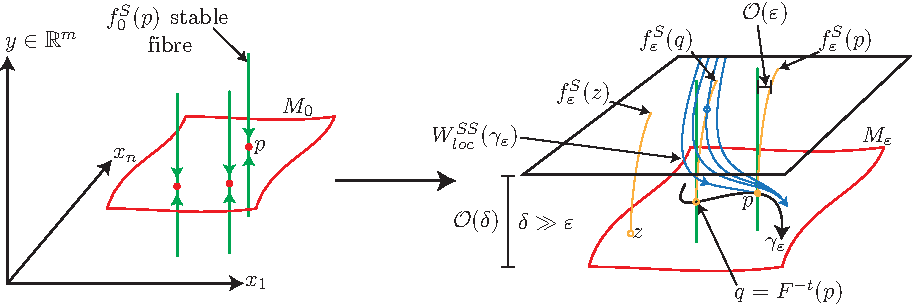
\includegraphics[width=0.99\textwidth]{figures/ch9/19perturbed_features.pdf}
	\caption{The dynamics near the slow manifold and the stable fibers with their relationship to $M_0$ and the stable fibers of the linearization.}
	\label{fig:perturbed_features}
\end{figure}

Define the $m+1$-dimensional \emph{strong stable manifold} of $\gamma_{\varepsilon}$ to be
\begin{align}
	W_{ \textrm{loc} }^{SS}(\gamma_{\varepsilon}) = \bigcup_{p \in \gamma_{\varepsilon}}f_{\varepsilon}^{S}(p),
\end{align}
i.e. the collection of fastest-converging trajectories to $\gamma_\varepsilon$. By construction, the stable fibers form an invariant family along $\gamma_{\varepsilon}$, i.e. $F^{t}(f^{S}_{\varepsilon}(q)) \subset f^{S}_{\varepsilon}(p)$.

\begin{ex}[Clustering of inertial particles in fluids]
	When finite-size inertial particles are suspended in fluids they tend to form clusters, even in incompressible fluids (as opposed to fluid particles). For a specific case, consider the steady flow in the wake of a bluff body \cite{Burns1999}. This can be seen in Fig. \ref{fig:vortex_street}.
\begin{figure}[h!]
	\centering
	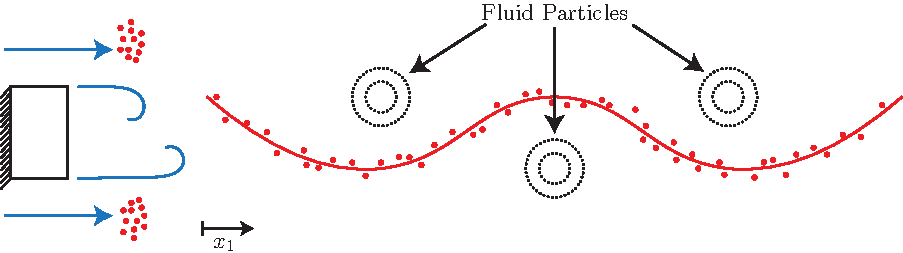
\includegraphics[width=0.99\textwidth]{figures/ch9/20vortex_street.pdf}
	\caption{The clustering of inertial particles observed experimentally, referred to as the \emph{von Kármán vortex street}.}
	\label{fig:vortex_street}
\end{figure}

The notation here will be $x\in \mathcal{S}^{1}\times \mathbb{R}$ for the particle position in a moving frame and periodic in the first variable. The steady fluid velocity in the moving frame is given by $u(x) \in \mathbb{R}^{2}$, the nondimensionalized particle mass is given by $\varepsilon \ll 1$, and the velocity of the inertial particle at time $t$ given by $y=\dot{x}\in \mathbb{R}^{2}$. The equation of motion in its simplest form is given by \cite{Maxey1983}
\begin{align}
	\begin{dcases}
		\dot{x} &=y\\
		\varepsilon \dot{y} & = u(x) - y
	\end{dcases}
	.
\end{align}
Thus we have the slow variable $x$ and the fast variable $y$, performing the time transformation as before ($t = \varepsilon \tau$) we obtain
\begin{align}
\begin{dcases}
	x' = \varepsilon y \\
	y' = u(x) - y
\end{dcases}
.	
\end{align}
the $\varepsilon=0$ limit yields
\begin{align}
	\begin{dcases}
		x' = 0 \\
		y' = u(x) - y = g(x,y,0)
	\end{dcases}
	.
\end{align}
Hence, we get the critical manifold
\begin{align}
	M_0 = \left\{ (x,y)\in U \subset \mathcal{S}^{1}\times \mathbb{R}^{3}:\ y = u(x)\right\}.
\end{align}
To examine the stability of $M_0$ calculate $D_{y}g(x, u(x), 0) = - I_{2}$, hence $ \textrm{Re} [\lambda_i]= \lambda_i =-1<0$ for $i=1,2$. Hence, $M_0$ is normally hyperbolic and attracting, the unperturbed fibers $f_{0}^{S}(p)$ for $p\in M_0$ are 2-dimensional planes. The unperturbed geometry is depicted in Fig. \ref{fig:unperturbed_fluid_geometry}.
\begin{figure}[h!]
	\centering
	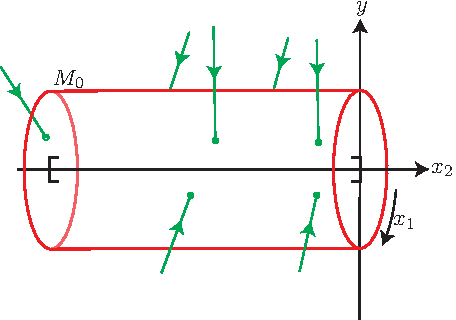
\includegraphics[width=0.6\textwidth]{figures/ch9/21unperturbed_fluid_geometry.pdf}
	\caption{The unperturbed geometry of the dynamics given in the example of inertial particles suspended in the fluid.}
	\label{fig:unperturbed_fluid_geometry}
\end{figure}

For $\varepsilon>0$ we get the perturbed manifold $M_{\varepsilon}$ which is $\mathcal{C}^{1}\ \mathcal{O}(\varepsilon)$-close to $M_0$. Trajectories in $W^{SS}(\gamma_{\varepsilon})$ quickly synchronize with $\gamma_{\varepsilon}$. The perturbed geometry is shown in Fig. \ref{fig:perturbed_fluid_geometry}.

\begin{figure}[h!]
	\centering
	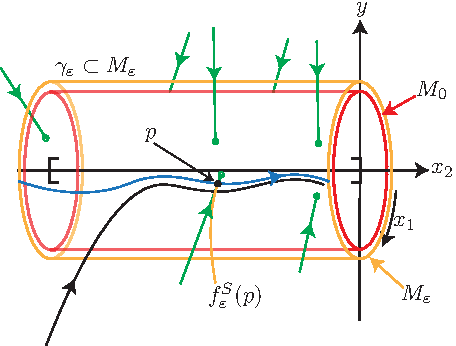
\includegraphics[width=0.6\textwidth]{figures/ch9/22perturbed_fluid_geometry.pdf}
	\caption{The perturbed geometry of the dynamics given in the example of inertial particles suspended in the fluid.}
	\label{fig:perturbed_fluid_geometry}
\end{figure}

To study the dynamics on the slow manifold, write the perturbed manifold $M_{\varepsilon}$ as the graph of the function $\varphi_{\varepsilon}$
\begin{align}
	M_{\varepsilon} = \left\{ (x,y):\ y=\varphi_{\varepsilon}(x)=\underbrace{\varphi_0(x)}_{u(x)} + \varepsilon h_{1}(x) + \mathcal{O}(\varepsilon^{2}) \right\}.
\end{align}

By the invariance of $M_{\varepsilon}$ the formula $y=\varphi_{\varepsilon}(x)$ holds along full trajectories. Plugging this in and differentiating with respect to $\tau$ we find
\begin{align}
	y' = (Du)x' + \varepsilon (Dh_{1})x' + \ldots = (Du) \varepsilon u(x) + \mathcal{O}(\varepsilon^{2}).
\end{align}
In the second equation the fact $x'=\varepsilon \varphi_{\varepsilon}(x)$ was used. Also from the equation of motion we find
\begin{align}
	\left. y'\right|_{M_{\varepsilon}} = \left. \left(u(x) - y\right) \right|_{M_{\varepsilon}} = u(x) - \left(u(x) + \varepsilon h_{1}(x) + \ldots\right) = - \varepsilon h_{1}(x) + \mathcal{O}(\varepsilon^{2}).
\end{align}
By comparing coefficients we then find
\begin{align}
	h_{1} = - (Du)u.
\end{align}
Hence, the reduced flow on the slow manifold is
\begin{align}
	x' = \varepsilon \varphi_{\varepsilon}(x) = \varepsilon \left( u(x) - \varepsilon (Du(x)) u(x) \right) + \mathcal{O}(\varepsilon^{2}).
\end{align}
Transforming this back into the original time we find
\begin{align}
	\dot{x} = u(x) - \varepsilon (Du(x))u(x) + \mathcal{O}(\varepsilon^{2}).
\end{align}
The $\mathcal{O}(1)$ term, $u(x)$, denotes the incompressible terms, meanwhile the $\mathcal{O}(\varepsilon)$ term is the dissipative terms (i.e. has nonzero divergence). This nonzero divergence can be calculated
\begin{align}
	\nabla \cdot \left[ (Du)u) \right] =  \textrm{Tr} \left[ Du Du\right] = - 2Q;\quad Q = \frac{1}{2}\left| \|\Omega\|^{2} - \| S\|^{2} \right|,
\end{align}
where $\| \cdot \|$ denotes the Euclidean matrix norm. The unperturbed system and $Q>0$ case are depicted in Fig. \ref{fig:clustering_Qpos}.
\begin{figure}[h!]
	\centering
	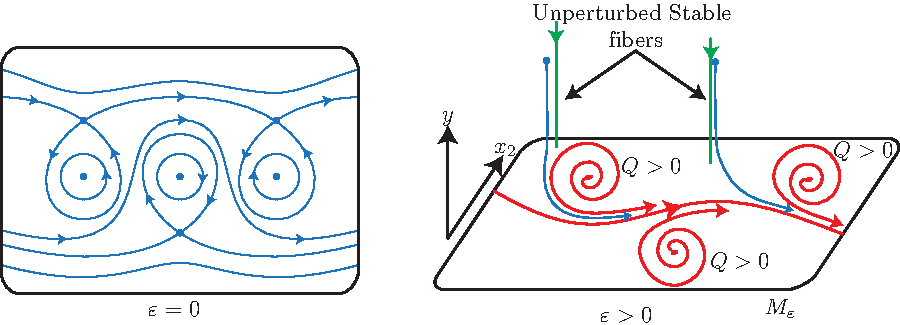
\includegraphics[width=0.99\textwidth]{figures/ch9/23Qpos_clustering.pdf}
%	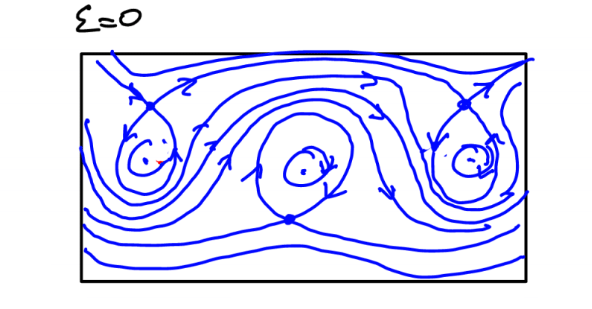
\includegraphics[width=0.45\textwidth]{figures/ch9/23a_Qpos_clustering.png}
%	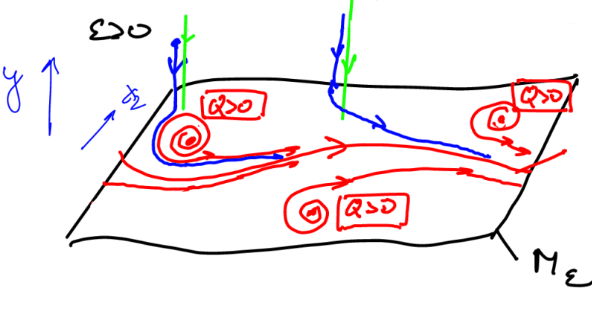
\includegraphics[width=0.45\textwidth]{figures/ch9/23b_Qpos_clustering.png}
	\caption{Left: The unperturbed phase space. Right: The perturbed phase space for $Q>0$, the green arrows denotes unperturbed stable fibers, and the red line designates the limit cycle. By identifying the left and right sides, we get a periodic variable.}
	\label{fig:clustering_Qpos}
\end{figure}

A more general approach to particle motion is given by \cite{Sapsis2008} using the Maxey-Riley equations. For neutrally buoyant particles (ones which are suspended in the fluid) we have
\begin{align}
	\varepsilon \dot{v} - \varepsilon \frac{Du}{Dt} = -(v-u);\quad \varepsilon = \frac{3St}{2}\ll 1, \label{eq9:maxeyriley}	
\end{align}
where $St$ denotes the Stokes number. Formulating this in terms of geometric singular perturbation theory, with $x \in \mathbb{R}^{d}$ ($d=2,3$) we get
\begin{align}
	\begin{dcases}
		\dot{x} = y\\
		\varepsilon \dot{y} = u(x,t) - y + \varepsilon \frac{Du(x,t)}{Dt}	
	\end{dcases}
\implies
\begin{dcases}
	t' = \varepsilon \\
	x' = \varepsilon y \\
	y' = u(x,t) - y + \varepsilon \frac{Du(x,t)}{Dt}
\end{dcases}
.
\end{align}
The time transformation used was $t = t_0 + \varepsilon \tau$. From here we have the slow variables $x$ and $t$, and the fast variable $y$. There then exists a $(d+1)$-dimensional slow manifold $M_\varepsilon$ where we have $y = u(x,t) + \varepsilon u_1(x,t) + \mathcal{O}(\varepsilon)$. The reduced particle dynamics here is given by
\begin{align}
	y' &= \nabla u x' + u_t \varepsilon + \varepsilon \nabla u_1 x' + u_{1t}\varepsilon^{2} + \mathcal{O}(\varepsilon^{2}) 
	= \varepsilon(\nabla uy + u_{t}) + \mathcal{O}(\varepsilon^{2}) \\
	   &= \varepsilon (\nabla u u + u_{t}) + \mathcal{O}(\varepsilon^{2}) 
	   = \varepsilon \frac{Du}{Dt} + \mathcal{O}(\varepsilon^{2}).
\end{align}
Also, we have 
\begin{align}
	y' &= u - \left( u + \varepsilon u_{1} + \mathcal{O}(\varepsilon^{2}) \right) + \varepsilon \left( u_{t} + u_{x}u \right) \\
	   &=-\varepsilon u_{1} + \varepsilon \frac{Du}{Dt} + \mathcal{O}(\varepsilon^{2}).
\end{align}
By  comparing terms we see that $u_{1} =0$, in fact this holds up to any order. 

The reduced dynamics on the slow manifold follow $\dot{x}=v=u(x,t)$ up to \underline{any} order independent of $\varepsilon$. This suggests a fast synchronization with the fluid, yet scattering of the particles is still observed along fluid motions. The reason for this can be seen by rewriting \eqref{eq9:maxeyriley}
\begin{align}
	\dot{v} - u_{t} - \nabla u u = \mu (u-v);\quad \dot{v} - u_{t} - \nabla u v = \mu (u-v) + \nabla u(u-v).
\end{align}
This implies that
\begin{align}
	\begin{dcases}
		\frac{d}{dt}\left(v - u(x,t)\right) = - \left( \nabla u + \mu I \right) \left( v - u \right) \\
		\frac{d}{dt} x = v
	\end{dcases}
	.
\end{align}
These in turn imply that $v=u(x,y)$ is an invariant manifold for any $\varepsilon = \frac{1}{\mu }$, but we only know its stability for $\varepsilon \ll 1$. 
This means that different parts of the manifold may have different stability types. 

To analyze the stability in more detail set $z= v- u(x,y)$, i.e. the distance from $ M_{\varepsilon} $ in the $y$-direction. The dynamics with this variable now is 
\begin{align}
	\begin{dcases}
		\dot{z} = - \left[ \nabla u(x,t) + \mu I \right] z \\
		\dot{x} = z + u(x,t)
	\end{dcases}
	\implies \frac{1}{2}\frac{d}{dt}\|z\|^{2} = - \langle z, (\nabla u + \mu I) z \rangle = - \langle z, (S + \mu I) z \rangle,
\end{align}
Where $S = \frac{1}{2} \left( \nabla u + \nabla u^{T} \right) = S^{T}$ is the rate of strain tensor.

We can derive conditions now for guaranteed attraction or repulsion:
\begin{enumerate}
	\item \textbf{Exponential attraction} is guaranteed when we have
		\begin{align}
			\frac{1}{2} \frac{d}{dt}\| z\| ^{2} \leq \lambda_{ \textrm{max} } \left[ -( S + \mu I) \right] \|z \|^{2}.
		\end{align}
		By the Gronwall-inequality, this implies
		\begin{align}
			\| z(t) \| \leq \| z(t_0)\| \exp\left( \int_{t_0}^{t} \lambda_{ \textrm{max} }[-(S + \mu I) ]ds \right).
		\end{align}
		Thus we have that $\|z(t)\|$ decays as long as we have
		\begin{align}
			\lambda_{ \textrm{max} }\left[ - S(x(t), y(t), t) - \mu I \right] < 0 
			\Leftrightarrow 
			\lambda _{ \textrm{min } } \left[ S(x,t) + \mu I \right] >0
			\Leftrightarrow
			\mu  > \sqrt{|\det(S)|}.
		\end{align}
	\item \textbf{Exponential repulsion} is guaranteed when we have  	
		\begin{align}
			\frac{1}{2} \frac{d}{dt}\| z\| ^{2} \geq \lambda_{ \textrm{min} } \left[ - (S + \mu I) \right] \|z \|^{2}.
		\end{align}
		Thus we have that $\|z(t)\|$ grows instantaneously when
		\begin{align}
			\lambda_{ \textrm{max} }\left[  -(S + \mu I) \right] > 0 \implies \lambda _{ \textrm{max} } \left[S + \mu I \right] < 0. 
		\end{align}
\end{enumerate}

More generally, an attracting/repelling invariant manifold may have localized repulsion/attraction along it, even if all trajectories approach it asymptotically \cite{Sapsis2010}.
\end{ex}

To study the local repulsion/attraction, consider the following dynamical system
\begin{align}
	\dot{x}= f(x,t);\quad x \in \mathbb{R}^{n},
\end{align}
with the flow map $F_{t_0}^{t}: x_0 \mapsto x(t;t_0, x_0)$ and a locally invariant $k$-dimensional manifold $\mathcal{M}(t) \subset \mathbb{R}^{n}$, i.e. $F_{t_0}^{t}(\mathcal{M}(t_0)) \subset \mathcal{M}(t)$. Now define the \emph{normal infinitesimal Lyapunov exponent} $\sigma(p,t)$ (abbreviated NILE) by taking the $t\to t_0$ limit and looking at the largest growth for a tangent vector $w_0$, i.e.
\begin{align}
	\boxed{
		\sigma(p,t) = \lim_{s\to 0} \frac{1}{s} \log \left\| \left.\Pi_{F_{t}^{t+s}(p)}^{t+s}DF_{t}^{t+s}(p) \right|_{N_{p}\mathcal{M}(t)} \right\|. 
		} \label{eq9:NILE_def}
\end{align}
The graphical depiction of the terms used for the calculation of the normal infinitesimal Lyapunov exponent are depicted in Fig. \ref{fig:NILE_def}.
\begin{figure}[h!]
	\centering
	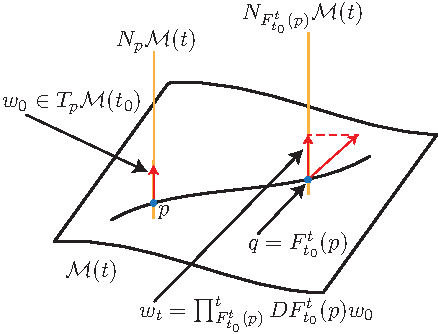
\includegraphics[width=0.6\textwidth]{figures/ch9/24NILE_def.pdf}
	\caption{The geometry of tangent vectors along the invariant manifold M. The quantities used to define the NILE \eqref{eq9:NILE_def} are indicated in the figure.}
	\label{fig:NILE_def}
\end{figure}

To compute the NILE we can use the following formula
\begin{align}
	\boxed{\sigma(p,t) = \max_{n\in N_{p}\mathcal{M}(t),\ |n|=1} \langle n, S(p,t)n\rangle;\quad S = \frac{1}{2}\left( Df + Df^{T}\right). }
\end{align}
Let us express the invariant manifold as a graph over $k$ variables, i.e. write $x$ as $x = (a,b)$, where $a \in \mathbb{R}^k$ and $b\in \mathbb{R}^{k-n}$, $f = (A, B)$ and on the invariant manifold $M$ we have $b = h(a)$. We can then write
\begin{align}
	\sigma(a,t) = \frac{1}{2}\lambda _{ \textrm{max} }\left[ \Gamma(a,t) + \Gamma(a,t)^{T} \right];
\end{align}
where we have defined the tensors
\begin{align}
	\Gamma(a,t)= B_{b} (a, h(a),t) - Dh(a,t) A_{b}(a, h(a),t).
\end{align}

\begin{ex}[Neutrally buoyant particles]
	Consider the dynamical system with $x,z\in \mathbb{R}^{2}$
	\begin{align}
		\begin{dcases}
			\dot{x} = z + u(x,t) \\
			\dot{z} = - \left( \nabla u(x,t) + \mu I \right) z
		\end{dcases}
		; \implies \mathcal{M}_{0}(t) \left\{ (x,z) \in \mathbb{R}^{2}\times \mathbb{R}^{2}:\ z =0\right\}.	
	\end{align}
Therefore we have 
\begin{align}
	\Gamma(a,t) = B_{b}(x,0,t) = - \left(\nabla u(x,t) + \mu I \right).
\end{align}
With this we can calculate the NILE
\begin{align}
	\sigma(p,t) = \lambda _{ \textrm{max} } \left[ - (S(x,t) + \mu I ) \right]; \quad S = \frac{\nabla u + \nabla u^{t}}{2}.
\end{align}
As concluded before, where $\sigma(p,t)>0$ we have a region of \underline{local} repulsion, analogously where $\sigma(p,t) <0$ we have a region of \underline{local} attraction.
\end{ex}

\section{Existence of invariant manifolds}
We now turn to the various methods to prove the existence of an invariant manifold:
\begin{enumerate}
	\item \textbf{Lyapunov-Perron Method} The manifold is the solution of a global integral equation, this approach requires global coordinates;
	\item \textbf{Hadamard's Method} The manifold is sought as an invariant graph, this was the approach Fenichel used and local coordinates are sufficient for this approach;
	\item \textbf{Topological Methods} There are multiple topological approaches, for instance the Wasewsky principle.
\end{enumerate}

Next, the Lyapunov-Perron method will be sketched for stable manifolds on the plane. Consider the dynamical system
\begin{align}
	\dot{x} = f(x);\quad x \in \mathbb{R}^{2};\quad f(0)=0;\quad  \textrm{spect} [Df(0)] = \{ - \lambda _{S}, \lambda _{U}\};\quad \lambda _S, \lambda_U > 0. \label{eq9:LP_method1}
\end{align}
The objective is to construct a stable manifold tangent to $E_{S}$. This will be achieved in multiple steps.
\begin{enumerate}
	\item First, choose a good basis
		\begin{align}
			x = Ty;\quad T = 
			\begin{pmatrix}
				e_{S} & e_{U}
			\end{pmatrix}
		;\quad y =
		\begin{pmatrix}
			y_S \\
			y_U
		\end{pmatrix}
		.
		\end{align}
	And implement this transformation 
	\begin{align}
		\dot{x} = Df(0)x + \mathcal{O}(\|x\|^{2}) \implies T\dot{y} = Df(0)Ty + \mathcal{O}(\| y\|^{2}).
	\end{align}
	By multiplying from the left by $T^{-1}$ we find
	\begin{align}
		\dot{y} = \underbrace{T^{-1}DF(0)T}_{ \textrm{diag} [-\lambda_S, \lambda_U ]}y + \mathcal{O}(\|y\|^{2});\quad \lim_{y \to 0} \frac{\|g(y)\|}{\|y\|^{2}}< \infty .
	\end{align}
	And now we find
	\begin{align}
		\begin{dcases}
			\dot{y}_{S} = - \lambda _{S}y_{S} + g_{S}(y) \\
			\dot{y}_{U} = \lambda _{U}y_{U} + g_{U}(y)
		\end{dcases}
		.
	\end{align}

\item Second, define the local stable manifold. The classic definition of $W^{S}(0)$ is that it is the collection of initial coordinates $y_0$ which under the limit of the flow map have $\lim_{t \to \infty }F_{t}(y_0)=0$. This requires detailed knowledge of asymptotics, and thus is hard to work with. For linear systems an alternative definition is, that $W^S(0)$ is the collection of forward-bounded trajectories, but this is generally nothing special after the addition of nonlinear terms. However, we may change the nonlinear system away from the origin to ensure that boundedness remains a distinguishing property. 

	To go about this we separate the phase space into the rectangular area (of half-width $\delta$) around the origin and the rectangular annulus of outer half-width $2\delta$. In the inner rectangle, the original nonlinear dynamics hold, outside of the annulus the dynamics are 0 (i.e. $f(x)=0$). Interpolating in between these regimes takes place on the annulus using a so-called \emph{bump function} $\Psi_{\delta}$, a smooth function which is equal to 1 on the interval $[-\delta, \delta]$ and equal to 0 on the intervals $(-\infty, -2\delta)$ and $(2\delta, \infty )$, in between these regions is the interpolation. The bump function and the interpolated new dynamical system are depicted in Fig. \ref{fig:interpolated_DS}.
\begin{figure}[h!]
	\centering
	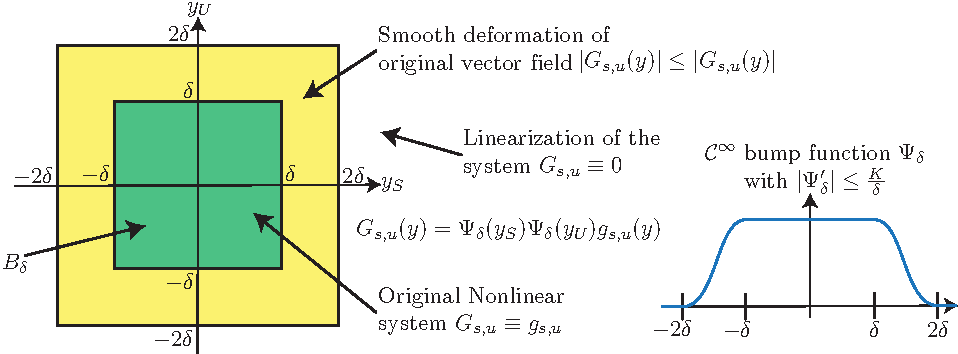
\includegraphics[width=0.99\textwidth]{figures/ch9/24_5interpolated_DS.pdf}
	\caption{The interpolated dynamical system, within the green area the original nonlinear dynamics hold, on the yellow area the smoothly deformed (interpolated) system holds, and outside of these two regions, the null dynamics hold. The bump function is also depicted.}
	\label{fig:interpolated_DS}
\end{figure}

Thus we have the modified system
\begin{align}
	\begin{dcases}
		\dot{y}_{S} = - \lambda_{S}y_{S} + G_{S}(y) \\
		\dot{y}_{U} = \lambda _{U} y_U + G_{U}(y)
	\end{dcases}
	.
\end{align}
Furthermore, we can bound this system
	\begin{subequations}
		\begin{align}
			|G'_{S,U}(y) | &= \Psi'_{\delta}g_{S,U} + \Psi_{\delta} g'_{S,U} \leq |\Psi_{\delta}| | g_{S,U}| + |\Psi_{\delta}| |g'_{S,U}|\\
				       &\leq \frac{K}{\delta} C \delta^2 + 1\cdot2\delta \leq C_0 \delta.	
		\end{align}
	\end{subequations}
	Then our goal becomes to find globally bounded solutions in the modified system, i.e.
	\begin{align}
		W^{S}_{ \textrm{loc} }(0) = \left\{ y_0 \in B_{\delta}:\ \sup_{t \geq 0}\left|\mathcal{F}^{t}(y_0) \right| < \infty \right\}.
	\end{align}

\item Now pretend that $y(t)$ is known to find the \emph{equivalent integral equations}. The variation of constants formula yields
	\begin{subequations}
	\begin{align}
		y_{S}(t) &= y_{S}(t_S) e^{- \lambda _{S}(t - t_S)} + \int_{t_S}^{t} e^{-\lambda _{S}(t-s)} G_{S}(y(s)) ds \\
		y_{U}(t) &= y_{U}(t_U) e^{ \lambda _{U}(t - t_U)} + \int_{t_U}^{t} e^{\lambda _{U}(t-s)} G_{U}(y(s)) ds. 
	\end{align}
	\end{subequations}
	By taking $t_{U}\to \infty $ and $t_{S}=0$ we restrict to $W^{S}_{ \textrm{loc} }(0)$, thus we find the integral equations for $W^{S}_{ \textrm{loc} }(0)$
	\begin{align}
		\begin{dcases}
		y_{S}(t) = e^{- \lambda _{s}t}y_{S}(0) + \int_{0}^{t} e^{-\lambda _{S}(t-s)}G_{S}(y(s))ds \\
		y_{U}(t) = \int_{\infty }^{t} e^{\lambda_{U}(t-s)}G_{U}(y(s))ds
		\end{dcases}
		.\label{eq9:LP_method5}		
	\end{align}
\item Finally we have a fixed point problem, the equation \eqref{eq9:LP_method5} is fulfilled when $y(t) = \mathcal{F}(y(t);y_S)$, thus we have a fixed point problem with the initial condition as a parameter. There exists a unique solution if $\mathcal{F}$ is a contraction mapping from a complete metric space into itself, i.e. when we can apply the Banach fixed point theorem. For $\mathcal{F}$ to be contracting, we require
	\begin{align}
		d(\mathcal{F}(x), \mathcal{F}(y)) \leq q d(x,y);\quad 0 < q < 1,
	\end{align}
for the metric $d$ defined over the underlying metric space.

Define the set
\begin{align}
	\mathcal{B}_{\delta} = \left\{ y(t): [0,\infty ) \to \mathbb{R}^{2}:\ y_{S}(0) = \delta,\ \|y\| \leq K,\ y\in \mathcal{C}^{0}[0, \infty ) \right\},
\end{align}
where the norm is $\|y\| = \sup_{t\geq 0}\|y(t)\|$. The space can be equipped with the metric 
\begin{align}
	d(x,y) = \sup_{t\geq 0} \| x(t) - y(t) \| = \| y - x\|,
\end{align}
and is complete with respect to this metric by the uniform convergence of Cauchy sequences of $\mathcal{C}^{0}$ functions to $\mathcal{C}^{0}$ functions, with limits obeying the same bound. We also have to show that $\mathcal{F}$ maps into itself, i.e. that $ \|\mathcal{F}(y) \| \leq K$ when $\|y\| \leq K$. To this end, calculate
\begin{subequations}
\begin{align}
	\|y(t)\| &\leq | y_{S}(t)| + |y_{U}(t) | \\
		 &\leq e^{-\lambda _{S}(t)}| y_{S}(0)| + \int_{0}^{t} e^{-\lambda _{S}(t-s)}{| G_{S}(y(s))|} ds + \int_{t}^{\infty } e^{\lambda _{U}(t-s)}{|G_{U}(y(s))|}ds \\
		 &\leq \delta + e^{-\lambda _{S}t}\int_{0}^{t} e^{\lambda _{S}s}\underbrace{| G_{S}(y(s))|}_{\leq C\delta^{2}} ds + e^{\lambda _{U}t}\int_{t}^{\infty } e^{-\lambda _{U}s}\underbrace{|G_{U}(y(s))|}_{\leq C\delta ^{2}}ds \\
		 &\leq \delta + C\delta^{2} \frac{1}{\lambda_{S}} \left[ e^{-\lambda _{S}(t-s)}\right]_{0}^{t} - \frac{C \delta^2}{\lambda _{U}} \left[ e^{\lambda _{U}(t-s)}\right]_{t}^{\infty } \\
		 &= \delta + C \delta^{2} \left( \frac{1}{\lambda_{S}}\left(1 - e^{-\lambda _{S}t}\right) + \frac{1}{\lambda _{U}}\left(1-0\right) \right) \\
		 &\leq \delta + C \delta^{2} \left( \frac{1}{\lambda _S} + \frac{1}{\lambda _U}\right) \leq K.
\end{align}
\end{subequations}
This shows that $y(t) \in \mathcal{B}_{\delta}$ for $\delta$ small enough. Furthermore, we have that $\mathcal{F}$ is a contraction mapping for $\delta$ small enough.
\begin{align}
	\|\mathcal{F}(y) - \mathcal{F}(x)\| &\leq \int_{0}^{t} e^{-\lambda_{S}(t-s)}| G_{S}(x(s)) - G_{S}(y(s))| ds \\
					    &\quad + \int_{t}^{\infty } e^{\lambda _{U}(t-s)} | G_{U}(x(s)) - G_{U}(y(s)) | ds \\
					    &\leq \int_{0}^{t} e^{-\lambda _{S}(t-s)}C_0 \delta \| x(s) - y(s)\| ds \\
					    &\quad + \int_{t}^{\infty } e^{\lambda _{U}(t-s)}C_0 \delta \|x(s) - y(s)\| ds \label{eq9:MVT}\\
					    &\leq C_0 \delta \left(\frac{1}{\lambda _{S}} + \frac{1}{\lambda _{U}} \right) \| x - y\|,
\end{align}
where in \eqref{eq9:MVT} the mean value theorem was used. This inequality implies that for $\delta$ small enough,
\begin{align}
	\|\mathcal{F}(y) - \mathcal{F}(x) \| \leq \underbrace{C_0 \delta \left( \frac{1}{\lambda_S} + \frac{1}{\lambda _{U}}\right) }_{\leq q < 1} \| x - y\|.
\end{align}
\end{enumerate}
For the general, mulit-dimensional case see \cite{Chicone}. A similar argument also work for the strong stable manifold.

\section{Spectral submanifolds and model reduction}
Often dynamical systems approach to model reduction. This leads us to want to identify globally attracting invariant sets $S$ and understand the reduced dynamics on said sets, i.e. the reduced order model. However, we must address the issue of the existence, uniqueness, and smoothness of these sets. Smoothness is not a given, as attractors are very often not smooth manifolds, as seen in Fig. \ref{fig:nonsmooth_set}.
\begin{figure}[h!]
	\centering
	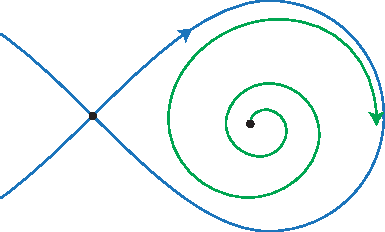
\includegraphics[width=0.6\textwidth]{figures/ch9/27nonsmooth_set.pdf}
	\caption{An example of a globally attracting set which is not a smooth manifold.}
	\label{fig:nonsmooth_set}
\end{figure}

In order to study these objects, we must first set out a few definitions.
\begin{definition}
	The \emph{global attractor} is the largest bounded, invariant, set (in forward and backward time) that attracts trajectories.
\end{definition}
\begin{definition}
An \emph{inertial manifold} is a lower-dimensional, attracting, forward-invariant manifold that is at least Lipschitz and contains the global attractor.
\end{definition}

The existence of inertial manifolds is not guaranteed in general, however the following proposition provides a sufficient condition \cite{FoiasInertial}.
\begin{proposition}[] \label{prop:FoiasExistence}
	If we have the dynamical system for a Hilbert space $H$
	\begin{align}
		\dot{u} = Au + R(u,u);\quad u\in H.
	\end{align}
Then given the following conditions:
\begin{enumerate}
	\item $A$ is self-adjoint, negative definite, and densely defined;
	\item $A^{-1}$ is compact;
	\item $R(u,u)$ is suitably dominated in norm by $Au$;
\end{enumerate}
then we have that the following hold:
\begin{enumerate}
	\item All trajectories enter a ball $B$ at some point;
	\item The timit set of the whole ball is the global attractor (inside the ball);
	\item An inertial manifold $M$ exists.
\end{enumerate}
Such a global attractor within a ball $B$ and the inertial manifold $M$ is depicted in Fig. \ref{fig:FoiaProp}.
\end{proposition}
\begin{figure}[h!]
	\centering
	\includegraphics[width=0.6\textwidth]{figures/ch9/FoiaProp.pdf}
	\caption{The red global attractor contained within the ball $B$ and the inertial manifold $M$ in the case of proposition \ref{prop:FoiasExistence}.}
	\label{fig:FoiaProp}
\end{figure}

An example in which such an $M$ is proven to exist can be found in the reaction-diffusion equation. In contrast, the proposition is not applicable to Navier-Stokes equations, even in 2 dimensions. Due to this restrictiveness we may insteade approximate the inertial manifold, following \cite{FoiasApprox}.

Assume we have the decomposition $u=p+q$ where $p$ is the projection $Pu$ of $u$, and $q$ is the residual after projection $q=(I-P)u$. We envision $p$ to be the slow variable and $q$ to be the fast variable. Using the self-adjointness of $A$, we obtain the projected equations
\begin{align}
	\begin{dcases}
		\dot{p} = Ap + PR(p+q, p+q) \\
		\dot{q} = Aq + (I-P)R(p+q, p+q).
	\end{dcases}
\end{align}

Next, we mimick geometric singular perturbation theory and set $\dot{p}=0$ which implies that $p$ is constant $p=p_0$. Therefore we get that the solutions to
\begin{align}
	Aq - (I-P)R(p_0 + q, p_0 +q) =0
\end{align}
yield the critical manifold. Next if we assume that $R(p_{0}+q, p_{0}+q) \approx R(p_0, p_0)$ then we find
\begin{align}
	q = \phi_0(p) = - A^{-1}(I-P)R(p,p).
\end{align}
The aim here is similar to critical manifold, and it should be kept in mind that we have relied on strong assumptions.

Now we may examine the simplest setting for a nonlinear model reduction, namely reduction near a fixed point in finite dimensions. Given the dynamical system
\begin{align}
\dot{x} = Ax + f(x);\quad x \in \mathbb{R}^{n},\ A \in \mathbb{R}^{n\times n},\ f\in \mathcal{C}^{r},\ f=\mathcal{O}\left(\|x\|^{2}\right).
\end{align}
Assume that $x=
\begin{pmatrix}
	x_s \\ X_f
\end{pmatrix}
$ where $x_s$ is aligned with the $s$ slower decaying modes and $x_f $ is aligned with the $f$ faster decaying modes. This enables us to write
\begin{align} \label{eq9:approx_inert_mfd}
	\begin{dcases}
		\dot{x}_s = A_{s}x_{s} + f_s(x_s, x_f) \\
		\dot{x}_f = A_{f}x_{f} + f_f(x_s, x_f). 
	\end{dcases}
\end{align}
In the simplest form, this entails a 2-dimensional dynamical system with $
\begin{pmatrix}
	x_s \\ x_f
\end{pmatrix}
=
\begin{pmatrix}
	x \\y
\end{pmatrix}
$ and the operators $f=0$ and $A_s,A_f = -a,-b$ where $0<a<b$. This case is illustrated in Fig. \ref{fig:simplestReduction}. The solutions of this system are
\begin{align}
	\begin{dcases}
		x(t) = x_0 e^{-at} \\
		y(t) = y_0 e^{-bt}.
	\end{dcases}
\end{align}
A family of attracting, invariant, manifolds if formed by this solution namely the solutions to
\begin{align}
	\frac{1}{a}\log\left(\frac{x}{x_0}\right) =\frac{1}{b}\log\left(\frac{y}{y_0}\right)
\end{align}
The solution is given in this case by $y = C x^{\frac{b}{a}}$, which is generally only $\lfloor \frac{b}{a} \rfloor$-times differentiable except when $C=0$ in which case the manifold is $\mathcal{C}^{\infty }$.
\begin{figure}[h!]
	\centering
	\includegraphics[width=0.6\textwidth]{figures/ch9/simplestReduction.pdf}
	\caption{An example of the simplest setting for a nonlinear model reduction.}
	\label{fig:simplestReduction}
\end{figure}

The reduced dynamics is the same on all of these invariant manifolds, namely
\begin{align}
	\dot{x} = -ax.
\end{align}

The conclusions are similar for general $n\geq 1$ in \ref{eq9:approx_inert_mfd} as long as $f(x) = 0$. Now we may ask ourselves if it is possible to find similar low-dimensional attracting, invariant, manifolds for $f(x) \neq 0$? To this end the simplest approach is to use linearization theorems to relate the invariant manifolds of the $f(x)=0$ case to those of the $f(x) \neq 0$ case. These come in various forms
\begin{enumerate}
	\item Hartman-Grobman theorem: If $ \textrm{Re} (\lambda_j) \neq 0$ for $j=1,\ldots,n$ then there exists a $\mathcal{C}^{0}$ linearization, thus this is insufficient for constructing smooth manifolds.
	\item Hartman theorem: If $ \textrm{Re} (\lambda_j)<0$ for $j=1,\ldots,n$ and $f\in \mathcal{C}^{2}$ then there exists a $\mathcal{C}^{1}$ linearization. This is insufficient for any Taylor expansion and does not carry over the smoothness of any manifold smoother than $\mathcal{C}^{1}$ in the linearized system.
	\item Poincaré-Dulac theorem \cite{poincare1951}: If we have $ \textrm{Re} (\lambda_j)<0$ for $j=1,\ldots,n$, $f\in \mathcal{C}^{a}$ and the following non-resonance condition holds
		\begin{align}
			\sum_{i=1}^{n} m_i \lambda_i \neq \lambda_j;\quad \forall m\in\mathbb{N}^{n}:\ \sum_{i-1}^{n} m_{i} \geq 2
		\end{align}
		then there exists a unique $\mathcal{C}^{a}$ linearization. In this case, all invariant manifolds of the linear part of \ref{eq9:approx_inert_mfd} continue to exist for $f(x)\neq 0$ without any change in their smoothness. It should be noted that the nonresonance condition still allows for 1:1 resonances, but no others.
	\item Strong Sterberg linearization theorem: Under all of the conditions of the Poincaré-Dulac theorem, but for $f\in \mathcal{C}^{r}$, then there exists a $\mathcal{C}^{r}$ linearization including the case of $r=\infty $. Under nonresonance, all $\mathcal{C}^{r}$ manifolds of the linearization continue to exists for $r \in \mathbb{N}^{+}\cup \{\infty \}$.
	\item Sterberg linearization theorem \cite{Sterberg1957}: With the same non-resonance theorem as above along with $f\in\mathcal{C}^{r}$ for $r \in \mathbb{N}^{+}\cup \infty $ then there exists a $\mathcal{C}^{\rho}$ linearization where $\rho\leq r$ and $\lim_{r\to \infty }\rho = \infty $. Note that this requires no assumptions on the eigenvalues as we had before. In the general non-resonant case, only $f\in \mathcal{C}^{\infty }$ gives specific enough linearization that preserves the smoothness of all invariant manifolds of the linearization.  
		
\end{enumerate}
\begin{remark}[]
	Note that the nonresonance condition implies hyperbolicity of the fixed point.
\end{remark}

In summary the results listed above guarantee that under sufficient non-resonance conditions the existence of various invariant manifolds tangent to eigenspaces even for the nonlinear system. These manifolds are called \emph{spectral submanifolds}.

We are now left with a few questions
\begin{enumerate}
	\item How do we compute spectral submanifolds in the nonlinear system?
	\item Which of the infinitely many submanifolds do we use for model reduction?
	\item As linearization of the full dynamics is more that what we need for model reduction, do such manifolds exist under less stringent conditions as well?
\end{enumerate}

To answer this we introduce the theory of (primary) spectral submanifolds and follow \cite{Ponsioen2016}. We begin by introducing the dynamical system
\begin{align}
	\dot{x} = Ax f_0(x),\ x \in \mathbb{R}^{n},\ f_{0}(x)=\mathcal{O}\left(\|x\|^2\right),\ f_0 \in \mathcal{C}^{r},
\end{align}
for $r \in \mathbb{N}^{+}\cup\{\infty , \textrm{a} \}$ where a signifies the $f_0$ being analytic. Note here that the first condition on $f_0$ implies that $x=0$ is a fixed point. The eigenvalues of $A$ given by $\lambda_1,\ldots,\lambda_N$ fulfill
\begin{align}
	\textrm{Re} (\lambda_n) \leq  \textrm{Re} (\lambda_{n-1}) \leq \ldots \leq  \textrm{Re} \lambda_1 	
\end{align}

This implies that $x=0$ is asymptotically stable. Assume that the eigenspaces are such that every eigenspace $E_j$ is the span of the real and imaginary parts of all eigenvectors and generalized eigenvectors corresponding to $\lambda_j$ for $j=1,\ldots,n$, thus we have
\begin{align}
\mathbb{R}^{n} = \bigoplus_{j=1}^{N}E_j	.
\end{align}
Such a set of eigenspaces is shown in Fig. \ref{fig:ponsioen_eigenspaces}.
\begin{figure}[h!]
	\centering
	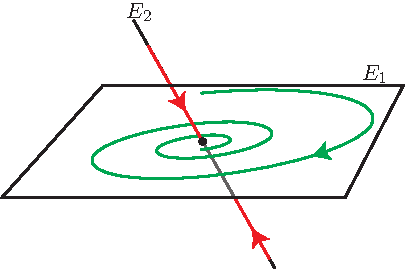
\includegraphics[width=\textwidth]{figures/ch9/30ponsioen_eigenspaces.pdf}
	\caption{A set of eigenspaces fulfilling the assumption that they are generated by the eigenvectors and generalized eigenvectors.}
	\label{fig:ponsioen_eigenspaces}
\end{figure}

Next we lay out a few definitions which will be useful for studying such dynamical systems.

\begin{definition}
We call the direct sum of an arbitrary number of distinct eigenspaces the \emph{spectral subspace} 
\begin{align}
E = \bigoplus_{j=1}^{t}E_{j};\quad 1 \leq k \leq N.	
\end{align}
This always forms an invariant subspace of $\dot{x}=Ax$.
\end{definition}
\begin{definition}

The \emph{spectral quotient of $A$} is given by
\begin{align}
	\sigma(E) = \left\lfloor \frac{ \textrm{smallest Re} [\lambda _k] \textrm{ outside of }E}{ \textrm{largest Re} [\lambda _i]  \textrm{ inside of } E}\right\rfloor.
\end{align}
An illustration of these two values are given in Fig. \ref{fig:spect_quotient}.
\begin{figure}[h!]
	\centering
	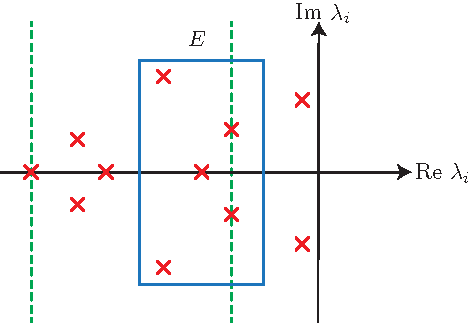
\includegraphics[width=0.6\textwidth]{figures/ch9/26spect_quot.pdf}
	\caption{The eigenvalue constellation, the left dotted green line designates the smallest real part outside of $E$ and the right dotted green line designates the largest real part inside of $E$.}
	\label{fig:spect_quotient2}
\end{figure}
\end{definition}

\begin{definition}
The \emph{external non-resonance condition for $E$} with $ \textrm{dim} [E]=q$ is
\begin{align}
	\langle m, \lambda \rangle_{E} = m_1 \lambda _{j1} + \ldots + m_1 \lambda _{jq} \neq \lambda_l,\ m_i \in \mathbb{N}	,
\end{align} 
where $\lambda _{j1},\ldots,\lambda _{jq}\in  \textrm{spect}[A|_{E}] $ and $\lambda _{l} \not \in  \textrm{spect} [A|_{E}]$.
\end{definition}

We proceed to ask ourselves if the full nonlinear system has a spectral submanifold (SSM), i.e. a nonlinear continuation of $E$.

\begin{theorem}[]
Assume the low-order external non-resonance condition
\begin{enumerate}
	\item $\langle m, \lambda \rangle_{E} \neq \lambda _l$ for $\lambda_l \neq  \textrm{spect}[A|_{E}] $;
	\item $2 \leq |m| \leq \sigma(E)$ with the norm $|m | =m_1 + \ldots + m_1$;
\end{enumerate}
then we have that the following hold:
\begin{enumerate}
	\item There exists a $\mathcal{C}^{r}$ spectral submanifold $W(0)$ tangent to $E$ at $x=0$ with the same dimension as $E$;
	\item $W(0)$ is unique among all $\mathcal{C}^{\sigma(E) + 1}$ invariant manifold satisfying (i);
	\item If $f_0$ is jointly $\mathcal{C}^{r}$ in $(x,\mu )$ for some parameter $\mu \in \mathbb{R}^{p}$, then so is $W(0)$, this also holds for $r=\infty $ and $r=a$. 
\end{enumerate}
Furthermore if $f_0$ is smooth or analytic in  $x$ and $\mu $, then so is $W(0)$.
\end{theorem}
\begin{proof}
	See \cite{Ponsioen2016}
\end{proof}
With this theorem, we can see that high-enough-order Taylor-series expansion puts us on $W(0)$ if we look for it as an invariant graph over $E$.

\begin{ex}[]
	Consider the dynamical system
	\begin{align}
		\begin{dcases}
			\dot{x} = - \frac{1}{4}x + xy + x^{3}\\
			\dot{y} = -y - 2x^2.
		\end{dcases}
	\end{align}
	These dynamics are depicted in Fig. \ref{fig:SSM_ex1}.
	\begin{figure}[h!]
		\centering
		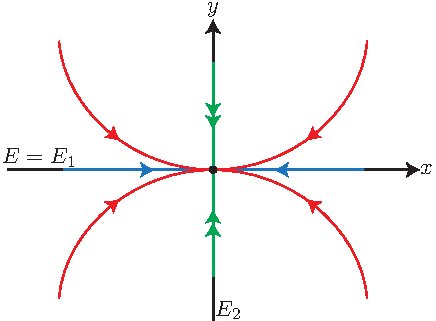
\includegraphics[width=0.6\textwidth]{figures/ch9/31ssm_ex1.pdf}
		\caption{The dynamics of the dynamical system given in the example.}
		\label{fig:SSM_ex1}
	\end{figure}	
	The slow spectral subspace is given by $E=E_1$ where $E_1$ is defined as the $x$-axis and can be seen in Fig. \ref{fig:SSM_ex1}. The spectral quotient of this manifold can be calculated
	\begin{align}
		\sigma(E) = \left\lfloor \frac{-1}{-\frac{1}{4}} \right\rfloor = 4.
	\end{align}
	It can also be seen that $m_1$ exists such that $m_1\lambda_1 = -m_1 \frac{1}{4} = -1 = \lambda_2 $ with $2 \leq |m| =m_1 \leq 4$, namely $m_1=4$, therefore the non-resonance condition for $E$ is not fulfilled and no unique spectral submanifold as a nonlinear continuation of $E$ exists. This is because a nonlinear continuation of $E$ can be concluded to exist from the theorem.
	Hence, we modify the system to
	\begin{align}
		\begin{dcases}
			\dot{x} = -\frac{1}{\alpha } x + xy + x^{3}\\
			\dot{y} = -y - 2x^2
		\end{dcases};\quad
		\alpha \not \in \mathbb{N}^{+} -\{1\}.
	\end{align}
	With this modification we find that $\sigma(E) = \lfloor \alpha \rfloor$, the non-resonance condition fails if $-m_1 \frac{1}{\alpha } \neq 1$ for $2\leq m_1 \leq \lfloor \alpha \rfloor$, thus we can see why we need the restriction on $\alpha $. Assuming such an $\alpha $ we find that there exists a unique spectral submanifold in the class of $\mathcal{C}^{\lfloor \alpha \rfloor + 1}$.

	Next, we look for a spectral submanifold as a Taylor expansion over $E$, to do this write the manifold as
	\begin{align}
		y = ax^2 + bx^3 + cx^4 + \mathcal{O}(x^5) = h(x).
	\end{align}
	We can derive this to find
	\begin{align} 
		\dot{y} = h'(x)\dot{x} &= \left(2ax + 3bx^2 + 4cx^3 + \mathcal{O}(x^4)\right) \left( - \frac{1}{\alpha } x + xh(x) + x^3 \right) \\
				       &= -\frac{2a}{\alpha } x^2 - \frac{3b}{\alpha }x^3 - \frac{4h}{\alpha }x^4 + 2a(a+1) x^4 + \mathcal{O}(x^5). \label{eq9:uno} 
       \end{align}
       Alternatively we find
       \begin{align}
		\dot{y} =\left. -y \right|_{W_E(0)} - 2x^2 &= -\left(ax^2 + bx^3 _ cx^4 + \mathcal{O}(x^5)\right) - 2x^2\\
							   &= -(a+2)x^2 - bx^3 - cx^4 + \mathcal{O}(x^5). \label{eq9:dos}
	\end{align}
	By comparing \ref{eq9:uno} and \ref{eq9:dos} we can see
	\begin{align}
		\mathcal{O}(x^2)&:\quad \frac{2a}{\alpha } = a+2 \quad &&\implies a(2-\alpha ) = 2\alpha; \\ 
		\mathcal{O}(x^3)&:\quad \frac{3b}{\alpha } = b \quad &&\implies b(3-\alpha ) = 0;\\
		\mathcal{O}(x^4)&:\quad 2a(a+1)- \frac{4c}{\alpha }= -c \quad &&\implies c(4-\alpha )= 2a(a+1)\alpha .
	\end{align}
These equations cannot be solved when a resonance is present. Furthermore, below that order all manifolds have the same expansion.

We may select $\alpha =\frac{3}{2}$ which implies $\lambda_1 = -\frac{2}{3}$ and $\lambda _2 = -1$, thus we have that $a=6$, $b=0$, and $c= \frac{2a(a+1)\alpha }{\alpha -1}>0$. Hence the spectral quotient can be calculate as $\sigma(E) = \left\lfloor \frac{-1}{-\frac{2}{3}}\right\rfloor = 1$, and thus $W_E(0)$ is already unique among the class of $\mathcal{C}^{2}$ invariant manifolds. Based on this we can see that the second order Taylor expansion only exists for $W_E(0)$ 
\begin{align}
	y = bx^2 + cx^4 + \mathcal{O}(x^5).
\end{align}
We may now write the reduced dynamics
\begin{align}
	\dot{x} = - \frac{2}{3} x + x(6x^2+cx^4 + \mathcal{O}(x^5)) + x^3 = -\frac{2}{3}x + 7x^3 + \mathcal{O}(x^4).
\end{align}
From here we derive the leading order model
\begin{align}
	\dot{x} = x\left( -\frac{2}{3} + 7x^2\right)
\end{align}
which has two nontrivial fixed points at $x = \pm \sqrt{\frac{2}{21}}$. Now we may ask if the full system has fixed points, namely by attempting to solve
\begin{align}
	\begin{dcases}
		-\frac{2}{3} x + xy + x^3 = 0\\
		-y - 2x^2 = 0.
	\end{dcases}
\end{align}
By setting the condition implied from the second equation into the first we find
\begin{align}
	-\frac{2}{3}x - x(2x^2) + x^3 = 0 \implies x\left(-\frac{2}{3} - x^2 \right) =0. 
\end{align}
This implies that no fixed point exist outside of the origin! The first order approximation to {\color{blue}(of?)} the spectral submanifold may not suffice, but we have the opportunity to go to \emph{any} order, without increasing the dimension of the reduced order model.
\end{ex}

Following the results of the previous example, we now look to extending the spectral submanifold to non-autonomous (forced) dynamical systems. For this we will assume the setup with $0\leq \varepsilon \ll 1$
\begin{align}
	\dot{x} = Ax + f_0(x) + \varepsilon f_1(x, \Omega t, \varepsilon);\quad x \in \mathbb{R}^{n},\ A \in \mathbb{R}^{n\times n},\ f_0,f_1 \in \mathcal{C}^{r},\ f_0 = \mathcal{O}(\|x\|^2).
\end{align}
Further we assume that $\Omega = (\Omega_1,\ldots,\Omega_k)\in \mathbb{R}^{k}$ has rationally independent entries and that $f_1$ is $2\pi$-periodic in the $\Omega t$ arguments. Furthermore we assume that the real parts of the eigenvalues are ascending and all strictly less than 0, i.e. the system restricted to $\dot{x}=Ax$ is asymptotically stable (and hyperbolic). We are interested in the spectral subspace $E= \bigoplus_{i}=E_{i}$, the direct sum of eigenspaces forming a $q$ dimensional space with $q\leq n$. Expanding on the definition the spectral quotient, define the absolute spectral quotient 
\begin{align}
	\Sigma(E) = \left\lfloor \frac{ \textrm{smallest Re}(\lambda_i)  \textrm{ in spect} (A) }{ \textrm{largest RE} (\lambda _2)\textrm{ in spect} (A|_{E})} \right\rfloor
\end{align}

The extended phase space is given by $\mathbb{R}^{n} \times \Pi^{k}$ where the dynamics is 
\begin{align}
\begin{dcases}
	\dot{x} = Ax + f_0(x) + \varepsilon f_1(x, \phi, \varepsilon) \\
	\dot{\phi} = \Omega 
\end{dcases}
;\quad \phi = \phi_0 + \Omega(t-t_0) \in \Pi^{k}.
\end{align}
The geometry of this system for $\varepsilon=0$ is shown in Fig. \ref{fig:ssm_eps0}.
\begin{figure}[h!]
	\centering
	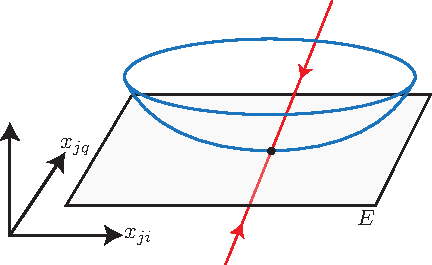
\includegraphics[width=\textwidth]{figures/ch9/32ssm_ex0.pdf}
	\caption{The geometry of the $\mathbb{R}^{k}$ portion of the dynamical system}
	\label{fig:ssm_eps0}
\end{figure}
\begin{theorem}[]
If we have that $\langle m, \lambda \rangle_E \neq \lambda_l$ for $2 \leq \|m\|_{1} \leq \sigma(E)$, $\lambda)i \in  \textrm{spect} (A|_{E})$, and $\lambda_l \in  \textrm{spect} (A)- \textrm{spect} (A|_{E})$, then the following hold for $\varepsilon >0$ small enough
\begin{enumerate}
	\item There exists a unique $\mathcal{C}^{r}$ invariant torus $T_{\varepsilon}$ ;
	\item There exists a unique spectral submanifold $W_{E}(T_{\varepsilon})$ of dimension $q+k$ which is $\mathcal{O}(\varepsilon)$ $\mathcal{C}^{r}$-close to $W_{E}(0)\times T_0$;
	\item $W_{E}(T_{\varepsilon})$ is already unique among all $\mathcal{C}^{\Sigma(E) + 1}$ invariant manifolds satisfying (ii);
	\item If $f_0$ and $f_1$ are smooth or analytics, then so is $W_{E}(T_\varepsilon)$ in $\varepsilon$ too.
\end{enumerate}
\end{theorem}
\begin{remark}[]
	Note that the non-resonance condition here is stronger than the previous, and is already violated when the real part of the spectrum has an outer resonance.
\end{remark}

\begin{ex}[]
	Consider the dynamical system
	\begin{align}
		\begin{dcases}
			\dot{x} = -x \\
			\dot{y} = -\sqrt{24}y + \underbrace{x^2 + X^3 + x^4 + x^5}_{f_0} + \underbrace{\varepsilon(\sin(t) + \sin(\sqrt{2}t))}_{\varepsilon f_1}.
		\end{dcases}
	\end{align}
	Therefore we have $\Omega = (1,\sqrt(2))$, i.e. $k=2$. We have $E = E_1$ and $\Sigma(E) = \left\lfloor \frac{- \sqrt(24)}{-1}\right\rfloor = 4$, this already tells use that if it exists then $W_{E}(T_{\varepsilon})$ is unique in $\mathcal{C}^{5}$. Next we check that the non-resonance condition is satisfied
	\begin{align}
		\forall m_1\in\mathbb{N}^{+}: \quad m_1(-1) \neq - \sqrt{24}.
	\end{align}
	Thus we have that there exists a unique, invariant, 2 dimensional torus $T_{\varepsilon}$ which is $\mathcal{O}(\varepsilon)$ $\mathcal{C}^{r}$-close to $T_0=0\times\Pi^{2}$ and that there exists a unique spectral submanifold $W_{E}(T_{\varepsilon})$ which is 3 dimensional. Both $T_{\varepsilon}$ and $W_{E}(T_\varepsilon)$ are explicitly computable and are indeed unique in the appropriate sense. These are shown in Fig. \ref{fig:ssm_ex2}.
	\begin{figure}[h!]
		\centering
		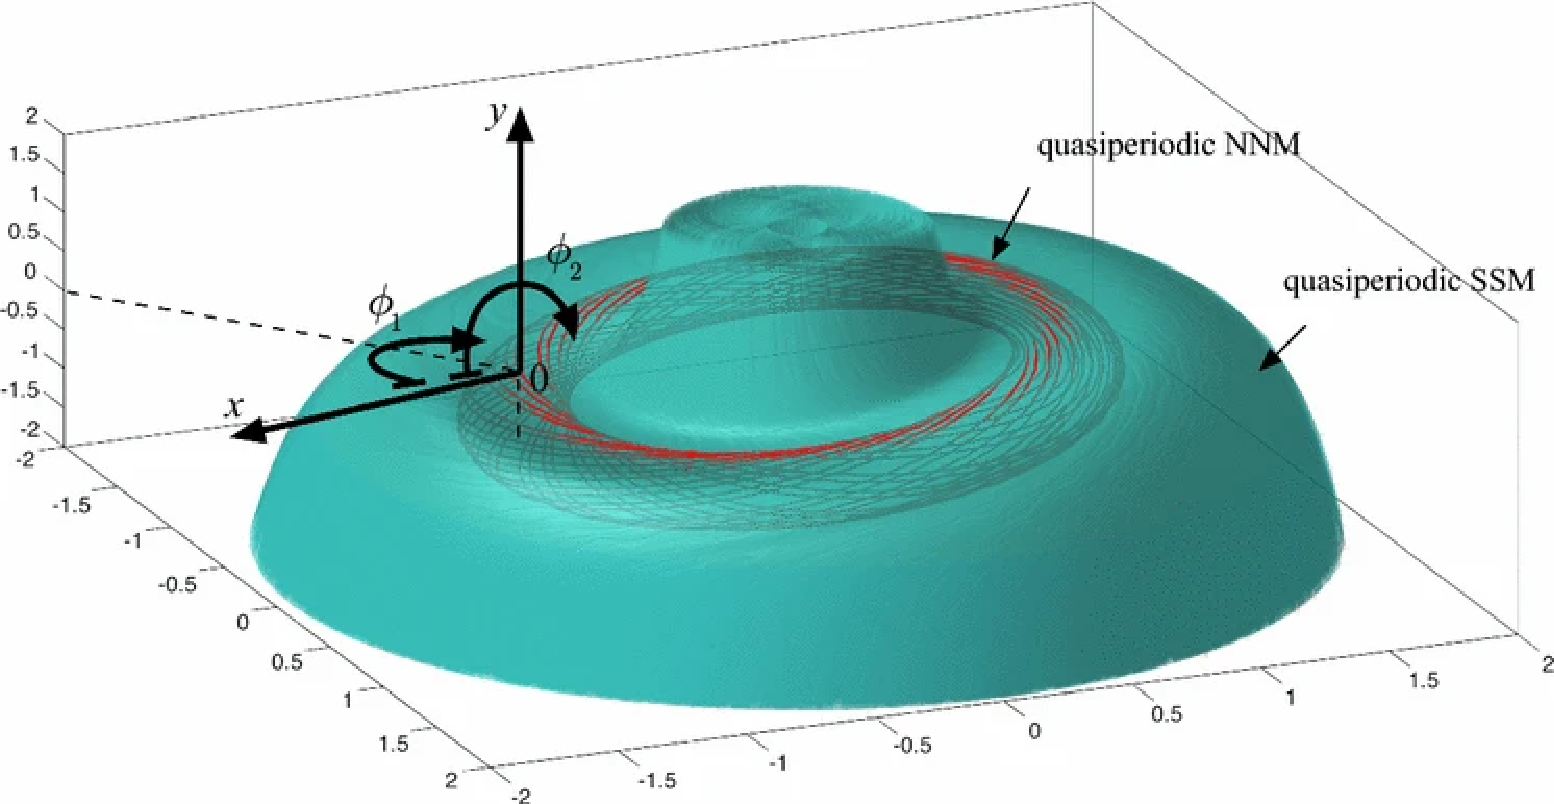
\includegraphics[width=0.6\textwidth]{figures/ch9/ponsioen2016.pdf}
		\caption{A projection of the extended phase space, the teal surface is the unique, analytic, quasiperiodic spectral submanifold, emanating from the unique quasiperiodic nonlinear normal mode in red \cite{Ponsioen2016}.}
		\label{fig:ssm_ex2}
	\end{figure}	
\end{ex}

We may now reduce the setting to mechanical systems, i.e. with $n$ degrees-of-freedom, damped-forced, weakly  nonlinear mechanical systems. Consider the dynamical system
\begin{align} \label{eq9:mech_ssm}
	M \ddot{q} + C \dot{q} + K q + N(q, \dot{q}) = \varepsilon F(q, \dot{q}, \Omega t, \varepsilon_);\quad q = 
	\begin{pmatrix}
		q_1 \\ \vdots \\q_n
	\end{pmatrix} \in \mathbb{R}^{n}.
\end{align}
Again we require that $F$ is quasi-periodic in the argument $\Omega t$ with rationally independent frequency vector $\Omega = (\Omega_1, \ldots, \Omega_k)$ with $\Omega_i\in\mathbb{R}^k$. The matrices $M$, $K$, and $C$ are all symmetric $\in \mathbb{R}^{n\times n}$ and are called the mass, stiffness, and damping matrices respectively, and all fulfill $M,K,C \succ 0$. 

The structural damping hypothesis states that $C = \alpha K + \beta M$, is convenient but is not required. Note that for $\varepsilon=0$ the eigenvalues of the linearization satisfy the characteristic equation $\det(\lambda^2 M + \lambda C + K) = 0$. This implies that $ \textrm{Re}(\lambda _{2n})\leq \ldots \leq  \textrm{Re} (\lambda _1) < 0$. For the linear system we have the Ansatz $q = e^{\lambda t}A$ for $A\neq 0$. The corresponding eigensolution (linear normal modes)
\begin{align}
	q_{j}(t) = \exp( \textrm{Re} (\lambda_j)t) \sin( \textrm{Im} (\lambda_j)t + \varphi_j) q_{0}^{j}.
\end{align}
The $j$-th mode shape is the constant vector $q_{0}^{j}\in \mathbb{R}^{n}$. If $ \textrm{Im} (\lambda_j) = 0$ we have an overdamped mode, otherwise if $ \textrm{Im} (\lambda _j)\neq 0$ we have an underdamped mode. The model coordinates are 
\begin{align}
	q=Tx,\ T = ( q_{0}^{1},\ldots, q_{0}^{n})	;\quad x \in \mathbb{R}^{n}.
\end{align}
In these coordinates \eqref{eq9:mech_ssm} becomes
\begin{align}
	\ddot{x}_{i}2 \xi_i\omega_i \dot{x}_{i} + \omega_{i}^{2}x_i + s_i(x, \dot{x}) = \varepsilon f_i(x, \dot{x}, \Omega t, \varepsilon).
\end{align}
The natural frequency $\omega_i$ is equal to $ \textrm{Im} (\lambda_i)$ and the modal damping factor $\xi_i$ is considering overdamping if $\xi_i >1$ and underdamped if $\xi_i<1$. The modal forcing terms are contained in $f_i$. Possible nonlinear responses are shown in Fig. \ref{fig:frf}.
\begin{figure}[h!]
	\centering
	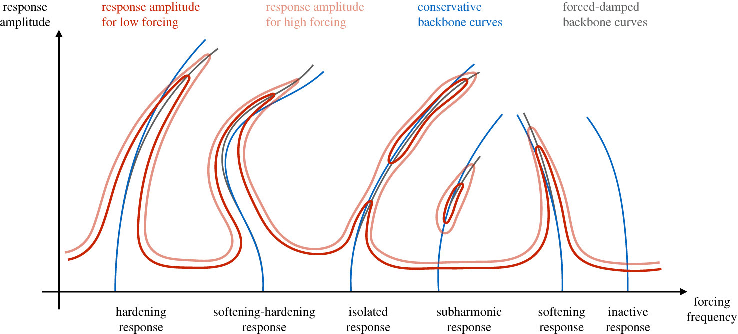
\includegraphics[width=0.99\textwidth]{figures/ch9/frf.pdf}
	\caption{Illustration of the frequency response phenomena in mechanical systems. The dark and ligh red curves identify the frequency response for low and high forcing amplitudes, respectively, while blue curves depict conservative backbone curves and grey curves represent force-damped backbone curves. \cite{Cenedese_2020}}
	\label{fig:frf}
\end{figure}

We can formulate this autonomously in the extended phase space $\mathbb{R}^{2n}\times \Pi^{k}$ 
\begin{align}
	\begin{dcases}
		\dot{x}_i = y_i \\
		\dot{y}_i = 2- \xi_i \omega_i y_i - \omega_i^2 x_i + S_i(x,y) +\varepsilon f(x,y,\phi, \varepsilon)\\
		\dot{\phi} = \Omega.
	\end{dcases}
\end{align}
The generalized quasiperiod spectral submanifold results apply here, for a typical forced response curve the forsing is periodic, $k=1$. The model subspace is the spectral subspace of the form $E=E_j$ with $E_j$ the eigenspace corresponding to the 2 eigenvalues of the $j$-th mode. Implied by the mode being overdamped, i.e. $\xi_j>1$, is that we only have negative real eigenvalues, thus the dynamics on $E_j$ form a node. Meanwhile in the underdamped case, we have a complex conjugate pair of eigenvalues, thus the dynamics on $E_j$ form a stable focus.  

The modal submanifolds are the nonlinear continuations of $E_j \times \Pi^{k}$ under forcing, i.e. the spectral subbundle of perturbed invariant tori $W_{E_j}(T_{\varepsilon})$. 
%We can observe an example of the geometry in Fig. \ref{fig:ssm_ex3}.

%\begin{figure}[h!]
%	\centering
%	%\includegraphics[width=\textwidth]{}
%	\caption{An example of the geometry of a nonlinear continuation of the extended phase space.}
%	\label{fig:ssm_ex3}
%\end{figure}

We may choose the dimension of the reduced order model (of the relevant spectral submanifold), this should be selected depending on how many of the transient time scales we would like to model (often stemming from the resonances with external forcing). Another consideration in this selection is that the lower-order internal resonances must be included in the spectral submanifold.

The most important case in nonlinear system id {\color{blue} what is this word?} and testing is with periodic external forcing ($k=1$, i.e. $T_0 \sim T_{\varepsilon} \sim S^1$). Of interest to us is predicting the forced response curve. Idealling we would find a nontrivial response near resonance which can be analyzed by reduction to $W_{E_j}(T_{\varepsilon})$. In this case $E_j$ is the modal subspace corresponding to the resonance.

The normal form for the reduced dynamics an 2 dimensional modal submanifolds is
\begin{align}
	\begin{dcases}
	\dot{\rho} = a(\rho) + \varepsilon (b_1(\rho, \Omega) \cos(\Psi) + b_2(\rho, \Omega)\sin(\Psi)) + \mathcal{O}(\varepsilon^2)\\
	\dot{\Psi} = b(\rho) - \Omega + \frac{\varepsilon}{\rho}(c_1(\rho, \Omega) \cos(\Psi) + c_2(\rho, \Omega)\cos(\Psi))+ \mathcal{O}(\varepsilon^2). 
	\end{dcases}
\end{align}
Where we have
\begin{align}
	a(\rho) &=  \textrm{Re} (\lambda_j) + \sum_{i}^{} a_i \rho^{2i+1} \\
	b(\rho) &=  \textrm{Im} (\lambda_j) + \sum_{i}^{} b_i \rho^{2i}, 
\end{align}
further $b_i$ and $c_i$ are Taylor series in $\rho$, which is convergend if $W_{E_j}(T_\varepsilon)$ is analytic. We call $\rho $ the polar radius, $\Psi $ the phase lag between the polar angle $\varphi $ and phase of the forcing, i.e. $\Psi = \varphi-\Omega t$. 
\begin{theorem}[]
	Nontrivial non-spurious transverse zeros of $a(\rho)$ (at $\rho_0$) give rise to isola, created around the point $(\Omega, \rho) = (b(\rho_0), \rho_0)$.
\end{theorem}
An illustration of the time periodic spectral submanifold and isola as in the theorem are given in Fig. \ref{fig:time_periodic_ssm}.
\begin{figure}[h!]
	\centering
	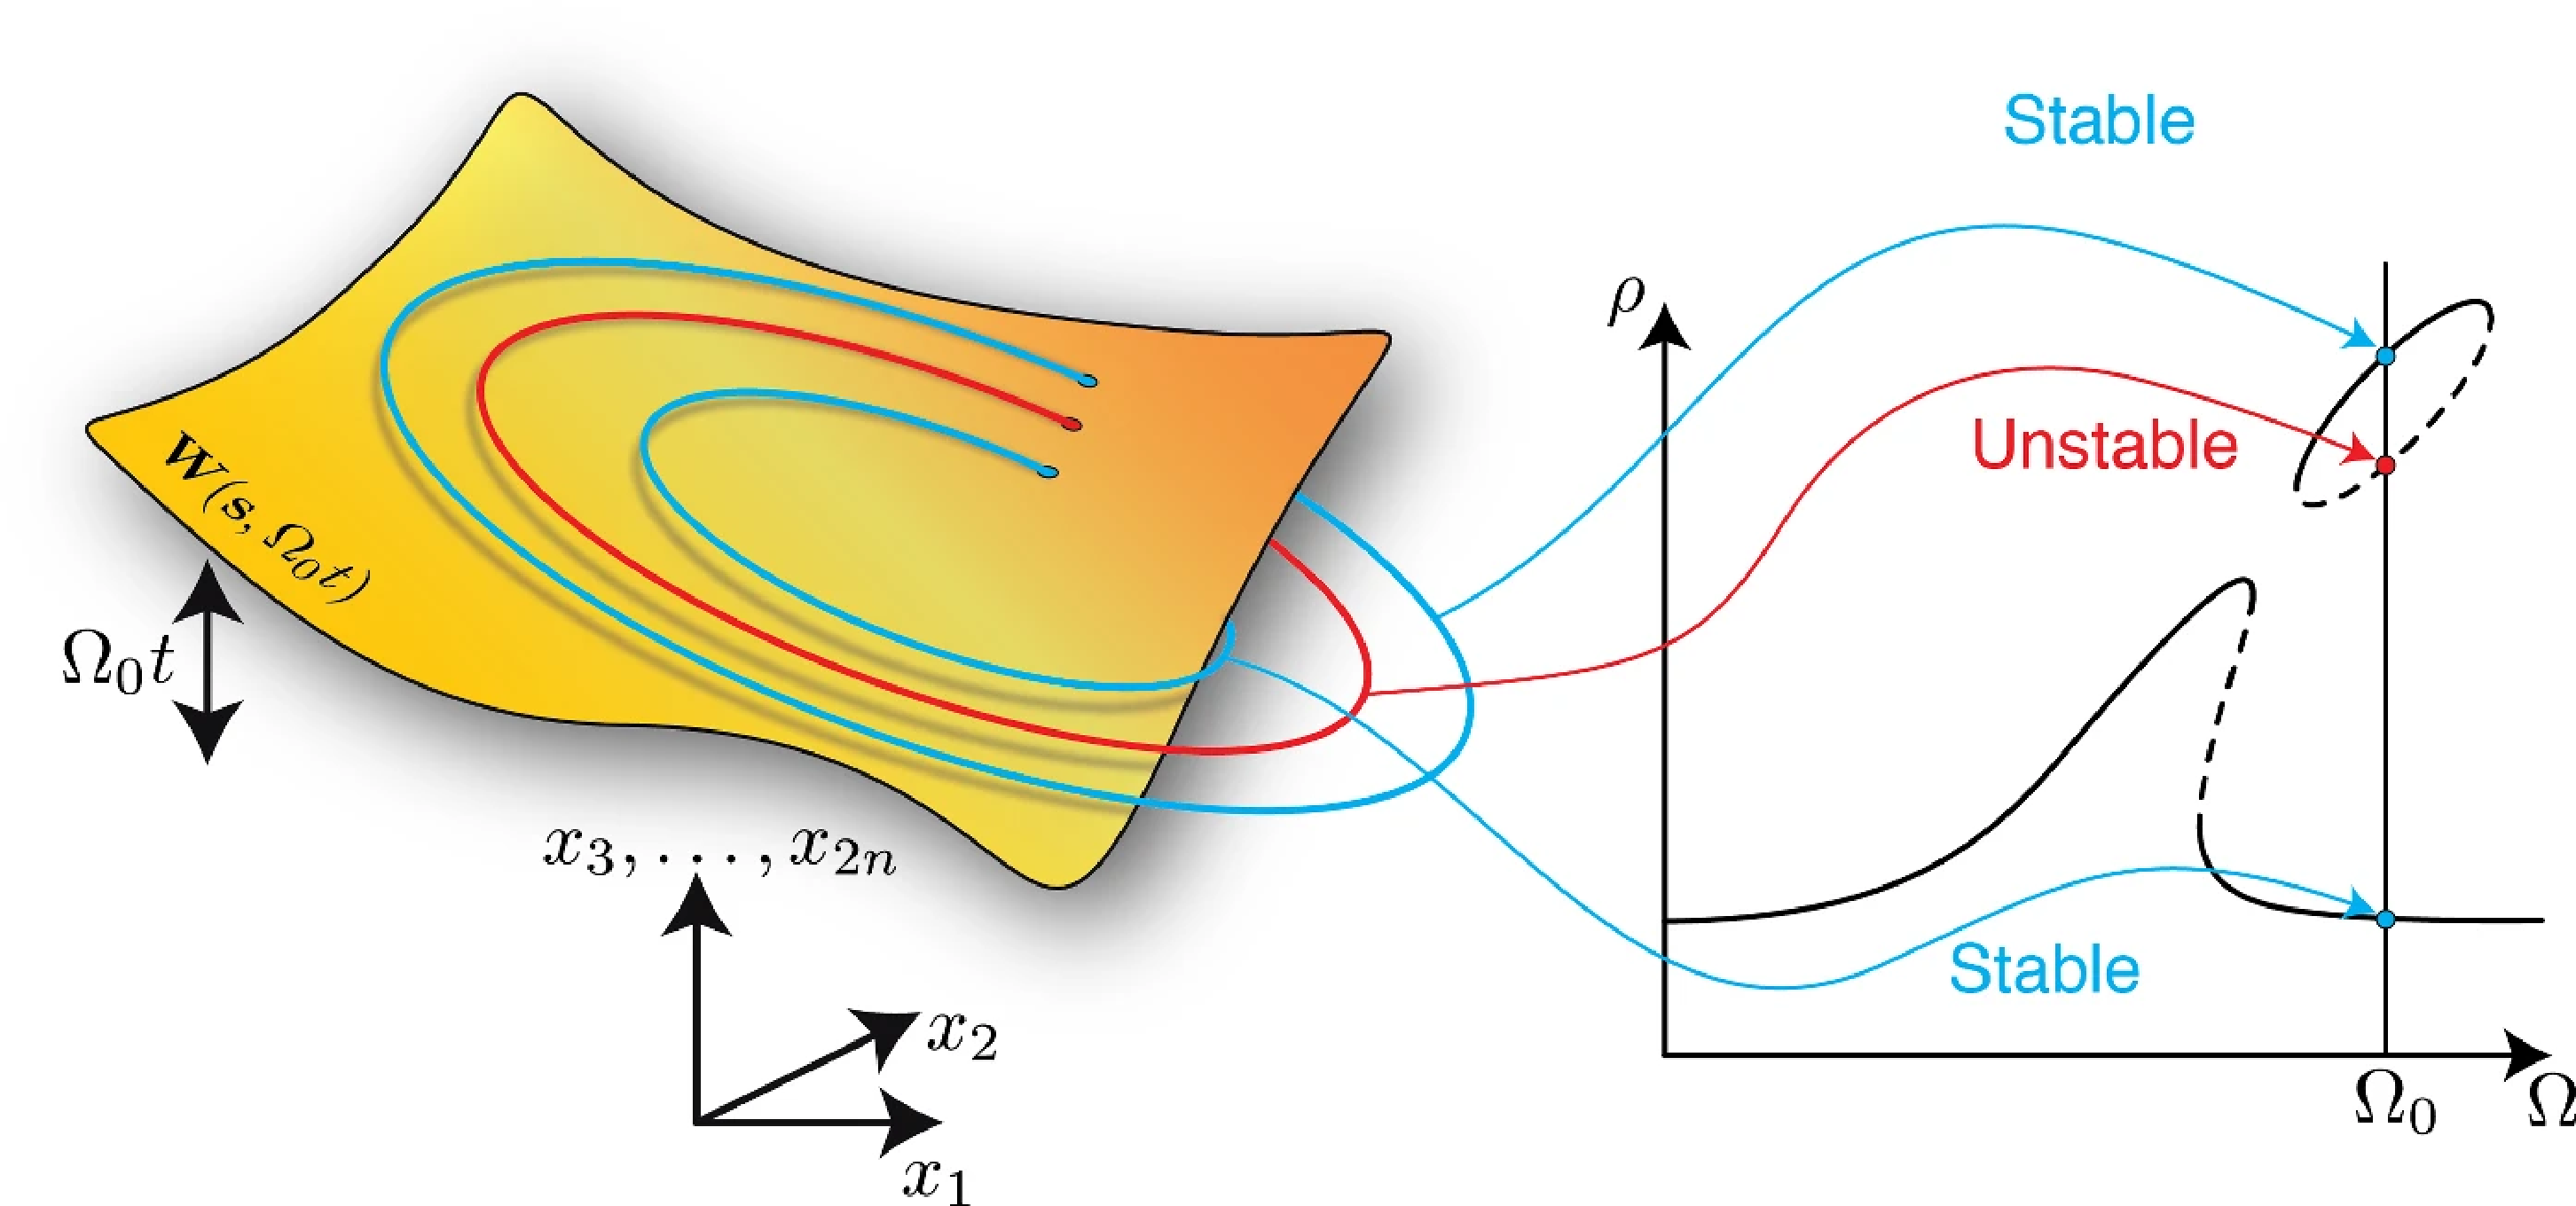
\includegraphics[width=0.6\textwidth]{figures/ch9/time_periodic_ssm.pdf}
	\caption{Illustration of a time periodic spectral submanifold. For a given forcing frequency $\Omega  $, here it is ullustrated how the spectral submanifold may contain three limit cycles, of which two fall in an isola \cite{Ponsioen2020}.}
	\label{fig:time_periodic_ssm}
\end{figure}


